% See section 11 of the User Manual for version history
%
%%%%%%%%%%%%%%%%%%%%%%%%%%%%%%%%%%%%%%%%%%%%%%%%%%%%%%%%%%%%%%%%%%%%%%
%%                                                                 %%
%% Please do not use \input{...} to include other tex files.       %%
%% Submit your LaTeX manuscript as one .tex document.              %%
%%                                                                 %%
%% All additional figures and files should be attached             %%
%% separately and not embedded in the \TeX\ document itself.       %%
%%                                                                 %%
%%%%%%%%%%%%%%%%%%%%%%%%%%%%%%%%%%%%%%%%%%%%%%%%%%%%%%%%%%%%%%%%%%%%%

%%\documentclass[referee,sn-basic]{sn-jnl}% referee option is meant for double line spacing

%%=======================================================%%
%% to print line numbers in the margin use lineno option %%
%%=======================================================%%

%%\documentclass[lineno,pdflatex,sn-basic]{sn-jnl}% Basic Springer Nature Reference Style/Chemistry Reference Style

%%=========================================================================================%%
%% the documentclass is set to pdflatex as default. You can delete it if not appropriate.  %%
%%=========================================================================================%%

%%\documentclass[sn-basic]{sn-jnl}% Basic Springer Nature Reference Style/Chemistry Reference Style

%%Note: the following reference styles support Namedate and Numbered referencing. By default the style follows the most common style. To switch between the options you can add or remove “Numbered” in the optional parenthesis. 
%%The option is available for: sn-basic.bst, sn-chicago.bst%  
 
%%\documentclass[pdflatex,sn-nature]{sn-jnl}% Style for submissions to Nature Portfolio journals
%%\documentclass[pdflatex,sn-basic]{sn-jnl}% Basic Springer Nature Reference Style/Chemistry Reference Style
\documentclass[pdflatex,sn-nature]{sn-jnl}% Nature Portfolio style (Scientific Reports)
%%\documentclass[pdflatex,sn-mathphys-ay]{sn-jnl}% Math and Physical Sciences Author Year Reference Style
%%\documentclass[pdflatex,sn-aps]{sn-jnl}% American Physical Society (APS) Reference Style
%%\documentclass[pdflatex,sn-vancouver-num]{sn-jnl}% Vancouver Numbered Reference Style
%%\documentclass[pdflatex,sn-vancouver-ay]{sn-jnl}% Vancouver Author Year Reference Style
%%\documentclass[pdflatex,sn-apa]{sn-jnl}% APA Reference Style
%%\documentclass[pdflatex,sn-chicago]{sn-jnl}% Chicago-based Humanities Reference Style

%%%% Standard Packages
%%<additional latex packages if required can be included here>
\usepackage{multirow}
\usepackage{makecell}
\usepackage{graphicx}%
\usepackage{multirow}%
\usepackage{amsmath,amssymb,amsfonts}%
\usepackage{amsthm}%
\usepackage{mathrsfs}%
\usepackage[title]{appendix}%
\usepackage{xcolor}%
\usepackage{float}
\usepackage{textcomp}%
\usepackage{manyfoot}%
\usepackage{booktabs}%
\usepackage{enumitem}
\usepackage{algorithm}%
\usepackage{algorithmicx}%
\usepackage{algpseudocode}%
\usepackage{listings}%
\usepackage{longtable}% not in template
\usepackage{makecell}% not in template
\usepackage{multirow}
\usepackage{placeins}
\usepackage[normalem]{ulem}
\graphicspath{{figures/}{paper/figures/}}

%%%% Revision highlighting (Scientific Reports resubmission) %%%%
% New or rewritten text is blue, removed text is struck through in red.
% Set \highlightfalse to produce the clean version for submission.
\newif\ifhighlight
\highlighttrue
\newcommand{\rev}[1]{\ifhighlight{\color{blue}{}#1}\else#1\fi}% the {} keeps a leading space
\newcommand{\revdel}[1]{\ifhighlight{\color{red}\sout{#1}}\fi}
\newcommand{\revnote}[1]{\ifhighlight{\color{magenta}\textbf{[#1]}}\fi}
%%%%

%%%%%=============================================================================%%%%
%%%%  Remarks: This template is provided to aid authors with the preparation
%%%%  of original research articles intended for submission to journals published 
%%%%  by Springer Nature. The guidance has been prepared in partnership with 
%%%%  production teams to conform to Springer Nature technical requirements. 
%%%%  Editorial and presentation requirements differ among journal portfolios and 
%%%%  research disciplines. You may find sections in this template are irrelevant 
%%%%  to your work and are empowered to omit any such section if allowed by the 
%%%%  journal you intend to submit to. The submission guidelines and policies 
%%%%  of the journal take precedence. A detailed User Manual is available in the 
%%%%  template package for technical guidance.
%%%%%=============================================================================%%%%

%% as per the requirement new theorem styles can be included as shown below
\theoremstyle{thmstyleone}%
\newtheorem{theorem}{Theorem}%  meant for continuous numbers
%%\newtheorem{theorem}{Theorem}[section]% meant for sectionwise numbers
%% optional argument [theorem] produces theorem numbering sequence instead of independent numbers for Proposition
\newtheorem{proposition}[theorem]{Proposition}% 
%%\newtheorem{proposition}{Proposition}% to get separate numbers for theorem and proposition etc.

\theoremstyle{thmstyletwo}%
\newtheorem{example}{Example}%
\newtheorem{remark}{Remark}%

\theoremstyle{thmstylethree}%
\newtheorem{definition}{Definition}%

\raggedbottom
%%\unnumbered% uncomment this for unnumbered level heads

\begin{document}

\title[Article Title]{
Comparative Study of Anatomical and Learned Features in AI Models for Structural Brain MRI%From Anatomical to Learned Features and Back: A Comparative Study of AI Models for Structural Brain MRI  
%Anatomy Guided Pre-Training for Structural Brain MRI
}

%%=============================================================%%
%% GivenName	-> \fnm{Joergen W.}
%% Particle	-> \spfx{van der} -> surname prefix
%% FamilyName	-> \sur{Ploeg}
%% Suffix	-> \sfx{IV}
%% \author*[1,2]{\fnm{Joergen W.} \spfx{van der} \sur{Ploeg} 
%%  \sfx{IV}}\email{iauthor@gmail.com}
%%=============================================================%%

\author[1]{\fnm{Boyang} \sur{Yu}}%\email{boy.yu@nyu.edu}


\equalcont{These authors contributed equally to this work.}

\author[1]{\fnm{Miquel} \spfx{Lopez} \sur{Escoriza}}%\email{miquel.lopez.escoriza@estudiantat.upc.edu }

\equalcont{These authors contributed equally to this work.}

\author[1,2]{\fnm{Long} \sur{Chen}}%\email{lc3424@nyu.edu}

\author[2]{\fnm{Arjun V.} \sur{Masurkar}}

\author[2]{\fnm{Narges} \sur{Razavian}}%\email{Narges.Razavian@nyulangone.org }

\author*[1,3]{\fnm{Carlos} \sur{Fernandez-Granda}}\email{cfgranda@cims.nyu.edu}


\affil[1]{\orgdiv{Center for Data Science}, \orgname{New York University, NYU}, \orgaddress{\street{60 Fifth Ave}, \city{New York}, \postcode{10011}, \state{New York}, \country{United States}}}

\affil[2]{\orgdiv{Department of Neurology}, \orgname{NYU Grossman School of Medicine}, \orgaddress{\street{ 550 1st Ave}, \city{New York}, \postcode{10016}, \state{New York}, \country{United States}}}

\affil[3]{\orgdiv{Courant Institute of Mathematical Sciences}, \orgname{NYU}, \orgaddress{\street{ 251 Mercer St}, \city{New York}, \postcode{10012}, \state{New York}, \country{United States}}}



%%==================================%%
%% Sample for unstructured abstract %%
%%==================================%%

% \abstract{The abstract serves both as a general introduction to the topic and as a brief, non-technical summary of the main results and their implications. Authors are advised to check the author instructions for the journal they are submitting to for word limits and if structural elements like subheadings, citations, or equations are permitted.}

%%================================%%
%% Sample for structured abstract %%
%%================================%%


\abstract{\rev{Artificial intelligence (AI) models for structural brain MRI obtain their features in three main ways: (1) computation of anatomical volumes, surface areas and cortical thicknesses, (2) supervised learning with convolutional neural networks (CNNs), and (3) self-supervised pretraining of vision transformer (ViT) foundation models followed by task-specific adaptation. We compare these paradigms on seven clinical tasks using 18 publicly available datasets comprising more than 96,000 T1-weighted MRI scans from approximately 80,000 participants, with evaluation on internal and external cohorts. A linear model based on anatomical features is competitive with CNNs and with ViTs pretrained on tens of thousands of scans across the diagnostic tasks. We further show that ViTs progressively encode anatomical information during self-supervised pretraining. Building on this observation, we propose Anatomy Segmentation Pretraining (ASP), which continues the pretraining of a masked-autoencoder ViT with brain-region segmentation as an auxiliary task. ASP performs on par with the other models on the diagnostic tasks and yields the most accurate brain age estimates, with the largest gains on two external cohorts. Our results establish anatomical features as a strong, interpretable baseline for structural MRI and indicate that explicit anatomical supervision can improve neuroimaging foundation models.}}
\keywords{Deep learning, pretraining, neuroimaging, brain anatomy, segmentation}

%%\pacs[JEL Classification]{D8, H51}

%%\pacs[MSC Classification]{35A01, 65L10, 65L12, 65L20, 65L70}

\maketitle

\section*{Introduction  }\label{intro}


\begin{figure}[h]
\makebox[\textwidth][c]{%
    \includegraphics[width=1.2\textwidth]{figures/figure_1.png}
}
\caption{\textbf{Overview of the study}. \textbf{(a) Cohorts used in the study.} Cohorts used for pretraining, downstream training, internal testing, and external evaluation. Reported $n$ values denote MRI scans; all splits were performed at the participant level, such that all scans from the same participant were assigned to the same split. External cohorts were drawn from independent data sources. \textbf{(b) AI models included in the study}. These represent the main feature-extraction approaches for neuroimaging data: linear models based on anatomical features, convolutional neural networks (CNNs) and vision transformers (ViTs) pretrained on large general-population cohort. For the ViTs, in addition to standard pretraining based on masked autoencoding, we propose a novel scheme called Anatomical Segmentation Pretraining (ASP).}
\label{fig:overview}
\end{figure}

Advances in machine learning and computer vision have exerted a major influence on neuroimaging over the past two decades. Initially, these models relied on hand-engineered features, such as hippocampal volume or cortical thickness, combined with classical statistical models (e.g. logistic regression or support vector machines)~\citep{kloppel2008automatic, wee2012identification,popuri2020using, hwang2022disentangling}. Subsequently, modern convolutional neural networks (CNNs) enabled automatic learning of complex features, which are challenging to interpret anatomically, but achieved strong performance for a variety of neuroimaging tasks ~\citep{payan2015predictingalzheimersdiseaseneuroimaging, basaia2019automated, chang2018deep, havaei2017brain}. More recently, foundation models based on vision transformers (ViTs) ~\citep{dosovitskiy2020image} are able to learn features from vast unlabeled datasets~\citep{caron2021emerging, he2022masked}. They can then be finetuned for different downstream tasks. Several recent works adapt this approach to neuroimaging data~\citep{hatamizadeh2022unetr, cox2024brainsegfounder, tak2024foundation,zhu20253d}, for example to develop multimodal models.

Several studies have explored incorporating anatomical information into brain MRI pretraining. QuickNAT\rev{~\citep{roy2019quicknat}} used automatically generated \rev{FreeSurfer} segmentation labels to \rev{pretrain} a neuroanatomical segmentation network\rev{, which was then finetuned on manual annotations}. API-MAE\rev{~\citep{wang2023improving}} incorporated \rev{an atlas-based} anatomical prior into the masking strategy of masked autoencoders\rev{ for tumor segmentation}, while DAMT\rev{~\citep{kim2024domain}} combined brain parcellation and morphological prediction with several self-supervised objectives\rev{ to pretrain a Swin transformer from scratch}. More recently, AnatCL\rev{~\citep{barbano2025anatomical}} leveraged regional anatomical measurements to guide contrastive representation learning. Together, these works establish the potential of anatomy-guided learning, but differ in the anatomical information used, the pretraining objectives, and the resulting representations. \rev{The approach proposed here differs from them in three respects. First, it is a continued-pretraining stage applied to an already converged masked autoencoder, in which segmentation alternates with masked-autoencoder updates so that the self-supervised features are retained. Second, the segmentation is predicted from the global ViT embedding by a lightweight decoder without skip connections, so that the anatomical information must be encoded in the representation that is later used for downstream tasks. Third, a region prompt makes voxel-level supervision of many brain regions memory-efficient in 3D. A detailed comparison is provided in Supplementary Table~\ref{tab:related_work}.}

In this work, we perform a comparative study of AI models for neuroimaging, with a focus on 3D structural T1-weighted MRI scans. T1-weighted MRI is a standard imaging modality that enables visualization of anatomical detail at a high resolution and is a routine part of most clinical protocols. Figure~\ref{fig:overview} provides an overview of the study. We consider seven different clinical tasks: diagnostics of Alzheimer's disease, epilepsy, Parkinson's disease, identification of tumor IDH mutations, brain age prediction and segmentation of brain tumors and stroke lesions. Overall, we use 18 different publicly-available datasets with more than 96,000 MRI scans from approximately 80,000 participants for training and evaluation\rev{, including seven external cohorts for Alzheimer's disease and two external cohorts for brain age}. 

Our overarching goal is to compare the three main strategies to obtain features for AI-based modeling in neuroimaging: (1) extraction of preselected anatomical characteristics such as volumes and surfaces of brain regions, (2) supervised learning with convolutional neural networks, and (3) unsupervised pretraining of foundation vision transformers on large general-population cohorts, followed by supervised finetuning. As reported in the Results section, the three strategies yield similar performance across the different tasks. Our results indicate that preselected anatomical features \revdel{match}\rev{are competitive with} the diagnostic performance of complex nonlinear features learned by sophisticated AI frameworks, including foundation models trained on \rev{tens of} thousands of scans. Conversely, convolutional neural networks and pretrained vision transformers \revdel{learn features that implicitly capture relevant anatomical information, bypassing}\rev{operate directly on the images and bypass} the need for computationally intensive feature extraction\rev{, which takes about six hours per scan with FreeSurfer}. 

In the case of ViTs pretrained on a large general-population cohort, we show that anatomical information is learned already during the pretraining stage, when the learned features become increasingly predictive of different brain structures. Inspired by this observation, we propose a novel pretraining strategy  (Anatomy Segmentation Pretraining or ASP), which aims to incorporate explicit anatomical grounding in the training of neuroimaging foundation models. As described in the Methods section, this is achieved by forcing the model to perform segmentation of relevant brain structures during pretraining. While this approach performs on par with the other strategies across the clinical tasks, it \revdel{achieves superior performance in estimating biological age}\rev{yields the most accurate brain age estimates}, a task for which a larger number of training data is available\rev{, and its advantage is largest on the external cohorts}.

In summary, this comparative study demonstrates that explicit anatomical features remain competitive with representations learned by advanced deep learning models, particularly across clinical cohorts ranging from dozens to thousands of training examples. Furthermore, we introduce a \revdel{novel, }\rev{simple} anatomy-guided pretraining framework that explicitly leverages anatomical information to enhance the pretraining of neuroimaging foundation models.


% where the number of training data

% It is worth noting that in other computer vision tasks, the datasets are orders of magnitude larger, here the training cohorts have up to a few thousand subjects.  

% ViTs pretrained using a novel strategy (Anatomy Segmentation Pretraining, denoted ASP ViT) that leverages anatomical information extracted via segmentation from the scans in the pretraining cohort.

% We compare simple linear models based on anatomical features, CNNs and ViT. We show that the ViT implicitly learns anatomical information, but only to some extent. We then propose a novel method to infuse additional anatomical information into the model, by incorporating a pretraining step that forces it to segment brain regions. We perform the comparison on XXX datasets, emphasizing evaluation on external cohorts.

% Our results indicate that in the regime all these AI models perform similarly, with slight advantages for ViT models that are not statistically significant. Remarkably, simple linear models based on anatomical features perform similarly to very large state-of-the-art ViTs. This suggests that (1) anatomical information is very useful, and (2) the bottleneck is the data available to perform task-specific adaption. To confirm, for an age estimation task with more data we observe that ViTs are better, and that the proposed anatomical pretraining provides a significant advantage.   


% Structural MRI is an important imaging modality for diagnostics. Brain structural MRI is used for...
%  T1 MRIs are the most commonly acquired brain scans\citep{wardlaw2012systematic,tak2024foundation, sudlow2015uk} in both clinical practice and research settings due to their ability to provide detailed structural information about brain anatomy. These scans offer consistent and reliable imaging data across diverse patient populations and scanning protocols, making them more widely accessible and applicable for model training. T1-weighted images are sufficient for a broad range of applications such as brain morphometry\citep{sudlow2015uk, bookheimer2019lifespan, harms2018extending, taylor2017cambridge, rowland2004information}, disease classification\citep{petersen2010alzheimer, beekly2007national, marcus2007open, marcus2010open, lamontagne2019oasis}, and age prediction\citep{sudlow2015uk,tak2024foundation, bookheimer2019lifespan, harms2018extending, taylor2017cambridge, rowland2004information}. Their prevalence across hospitals and imaging centers ensures that models built on T1 MRIs can be generalized across various healthcare systems, enabling more scalable and efficient clinical solutions. Therefore, focusing on T1 MRI enables the development of a versatile and practical foundation model with widespread applicability and impact in neuroimaging.
 
% Multiple AI models have been proposed, inspired by advances in deep learning. First, handcrafted features. Then, convolutional neural networks. Now, vision transformers, which usually need to be pretrained on large datasets. 

% Here we consider several tasks: Alzheimer's diagnosis, Parkinson's disease detection, epilepsy detection, brain tumor mutation identification, healthy brain aging, brain tumor segmentation and stroke lesion segmentation. These tasks are evaluated across 15 additional datasets, as shown in Figure~\ref{fig:overview}. We compare linear models based on anatomical features consisting of brain-region volumes and surfaces, convolutional neural networks trained in a supervised manner, and vision transformers pretrained on ... Evaluation is carried out on independent external datasets. 

% MRI-based brain age prediction is associated with neurocognitive function~\citep{marin2024brain, lee2022deep, biondo2022brain} in aging adults and may have utility as an early biomarker for Alzheimer’s disease. 

% We observe that ViTs pretrained on a general population automatically learn anatomical information. We use the learned features to fit linear models of different volumes and surfaces during training. The accuracy increases, indicating that the features encode anatomical information. Inspired by this, we propose to perform further pretraining by incorporating a segmentation task. We alternate between MAE and segmentation. 

% We observe that the three strategies perform similarly for AD...


% TO BE COMMENTED OUT AFTER THIS, PLEASE CHECK IF YOU WANT TO SAVE ANY REFERENCES

%Foundation models, particularly in the context of healthcare and medical imaging\citep{zhu20253d, tak2024foundation, cox2024brainsegfounder, zhou2023foundation, chen2024towards, zhu2024medical, wang2023sam}, offer a promising solution to mitigate data scarcity, especially when high-quality labeled data is limited. These models, by leveraging self-supervised learning in pretraining\citep{oquab2023dinov2, caron2021emerging, he2022masked}, and targeted adaptation, enable the learning of generalized representations from large, unlabeled datasets. This allows for more scalable and robust solutions compared to traditional anomaly detection models, which often rely on the availability of high-quality labeled data and are tailored to specific tasks or diseases. Additionally, foundation models  can serve as the vision foundation for multimodal tasks by acting as a core component of larger frameworks that integrate data from multiple modalities\citep{bai2024m3d, blankemeier2024merlin, chen2024medblip}, offering flexibility and efficiency in real-world clinical settings. As a result, foundation models not only provide a scalable solution to the data scarcity problem but also unlock the potential for AI-driven healthcare applications across a wide range of medical imaging modalities and clinical tasks.

%Recently, there have been numerous efforts to build vision foundation models in the healthcare domain. However, many of these models take a very general approach, combining various types of medical imaging without providing sufficient context for each individual image modality\citep{bai2024m3d, blankemeier2024merlin, zhu2024medical, wang2023sam}. This broad approach has limitations, as highlighted by models like FM-CT\citep{zhu2024medical} and BrainIAC\citep{tak2024foundation}, which show that such models struggle to improve performance on modality-specific tasks.

%Previous studies have proposed foundation model frameworks tailored to specific downstream tasks, such as dense prediction tasks (e.g., brain lesion segmentation\citep{cox2024brainsegfounder, zhu2024medical, wang2023sam}) and whole-image prediction tasks (e.g., brain aging, tumor mutation, disease survival\citep{tak2024foundation, zhu20253d}). Models for whole-image prediction tasks focus on broader analyses, such as predicting brain aging, identifying tumor mutations, or assessing disease survival. For instance, some models trained for brain aging might analyze global features of brain structure, such as total brain volume, while models for disease survival prediction might focus on overall patterns and disease progression. However, these models are often specialized and limited to one type of task, and there remains a critical gap in the field for a more generalized foundation model capable of seamlessly handling both dense prediction tasks (like segmentation) and global prediction tasks (such as aging or disease progression). A unified model with this capacity could enable more flexible and efficient deployment in diverse clinical settings, allowing for better integration across different types of analysis.

%Many foundation models, while powerful, are often trained on internal datasets that come with significant limitations, primarily legal and access-related restrictions\citep{zhu20253d, yang2024advancing}. For example, models trained on private clinical datasets may face strict regulations surrounding data access and patient confidentiality\citep{berman2002confidentiality, price2019privacy, kaissis2020secure}, making them less accessible for broader research and application. Furthermore, these proprietary datasets can be limited in terms of diversity, which can hinder the generalization of the models across different patient populations or medical conditions\citep{arora2023value, zhu20253d, ong2024shortcut}. To address these challenges, we focus exclusively on public brain imaging datasets, such as those from UK Biobank (UKBB)\citep{sudlow2015uk}, Human Connectome Project (HCP) \citep{harms2018extending}, National Alzheimer's Coordinating Center (NACC)\citep{beekly2007national} and other, which are openly accessible and provide a rich source of data that spans a wide range of conditions and demographics. By using publicly available data, we ensure that our foundation models are more broadly applicable, enabling researchers and clinicians worldwide to use and build upon these models, ultimately fostering greater collaboration and progress in the field of brain imaging. This approach also reduces barriers to entry for institutions with limited access to proprietary datasets, promoting more equitable and inclusive advances in the use of AI in healthcare.

% In this study, we first curated BrainATLAS, a large and diverse collection of T1-weighted brain MRI datasets sourced exclusively from publicly available neuroimaging resources. The dataset includes 19 distinct imaging studies to ensure a wide variety of study populations. We then introduce NeuroVision, a comprehensive brain MRI foundation model built on vision transformer architecture\citep{dosovitskiy2020image}, leveraging self-supervised learning (SSL) principles. While SSL has demonstrated success in both natural image and general medical imaging tasks, training a robust 3D MRI volume encoder presents unique challenges, such as selecting appropriate pretext tasks, managing spatial normalization, and addressing the high computational demands\citep{zhu20253d}. To overcome these challenges, we developed a standardized pipeline that harmonizes MRI scans from various protocols, ensuring consistent input for the foundation model. For pre-training, we adapted a masked image inpainting strategy, inspired by Masked Autoencoders (MAE)\citep{he2022masked}, and tailored it for a customized 3D vision Transformer (ViT). Pre-training was conducted on a large cohort of 69,878 brain MRI scans from four public databases.

% \begin{figure}[t!]%
% \centering
% \includegraphics[width=0.7\textwidth]{figures/fig1_neurovision_overview.pdf}
% \caption{\textbf{Overview of NeuroVision study.} \textbf{a.}, Collection of training data from UK BioBank and other public neuroimaging sources. \textbf{b.} Pretraining of the foundation model with 3D ViT for masked image reconstruction task. \textbf{c.} Evaluation design of the foundation model using 15 distinct external datasets for image-level prediction and dense predict tasks.
% }\label{fig:neurovision_overview}
% \end{figure}

\begin{table}[t]
\caption{Datasets used to build the pretraining cohort, and the training and evaluation cohorts for each task in the study.\rev{ Scans and participants are counted after FreeSurfer quality control. $^{\dagger}$ATLAS R2.0 contains one scan per participant, acquired at 33 sites.}}
\label{tab:datasets}
\centering
\begin{tabular}{l|c|c|c|c|c}
\hline
\textbf{Dataset} & \makecell{Number of\\ scans} & \makecell{Number of\\ subjects} & \makecell{Age (years)\\ (mean ± std)}  & \makecell{Gender\\ (female \%)} & \makecell{Brain volume in mL\\ (mean ± std)} \\ \hline
UKBB & 67294 & 62665 & 64.93 ± 7.69 & 52.81\% & 1156 ± 114 \\ 
HCP & 1350 & 1350 & 38.66 ± 25.76 & 54.97\% & 1179 ± 137 \\ 
CamCAN & 653 & 653 & 54.2 ± 18.5  & 49.35\% & 1156 ± 128 \\ 
IXI & 581 & 581 & 48.65 ± 16.47 & 53.87\% & 1137 ± 131 \\ \hline
NACC & 6956 & 4926 & 71.41 ± 11.25 & 53.34\% & 1034 ± 185 \\ 
ADNI & 6471 & 1817 & 74.68 ± 7.64 & 47.45\% & 1072 ± 116 \\ 
AIBL & 1167 & 664 & 74.56 ± 6.79 & 52.87\% & 1078 ± 110 \\ 
OASIS1 & 436 & 416 & 51.35 ± 25.27 & 61.47\% & 1089 ± 153 \\ 
OASIS2 & 373 & 150 & 77.01 ± 7.64 & 57.10\% & 1045 ± 124 \\ 
OASIS3 & 2275 & 1044 & 70.69 ± 9.18 & 48.39\% & 1061 ± 113 \\ 
OASIS4 & 181 & 180 & 71.09 ± 9.60 & 46.96\% & 1060 ± 116 \\ 
MIRIAD & 705 & 69 & 69.65 ± 6.88 & 55.51\% & 1039 ± 115 \\ 
% NIFD & 637 & 303 &  64.73 ± 7.42 & 46.31\% & 1048 ± 167\\ 
PPMI & 2032 & 1306 & 63.29 ± 9.58 & 40.59\% & 1119 ± 157 \\ 
OpenNeuro & 163 & 163 & 6.67 ± 2.47 & 46.01\% & 1195 ± 144 \\ 
EPISURG & 268 & 268 & NA & NA & 1102 ± 133 \\ 
UCSF-PDGM & 1980 & 501 & 56.87 ± 15.02 & 40.32\% & NA \\ 
BraTS & 2502 & 1251 & NA & NA & 1103 ± 136 \\ 
ATLAS & 655 & \revdel{33}\rev{655$^{\dagger}$} & NA & NA & 1445 ± 124 \\ \hline
\end{tabular}
\end{table}

\begin{figure}[t]%
\centering
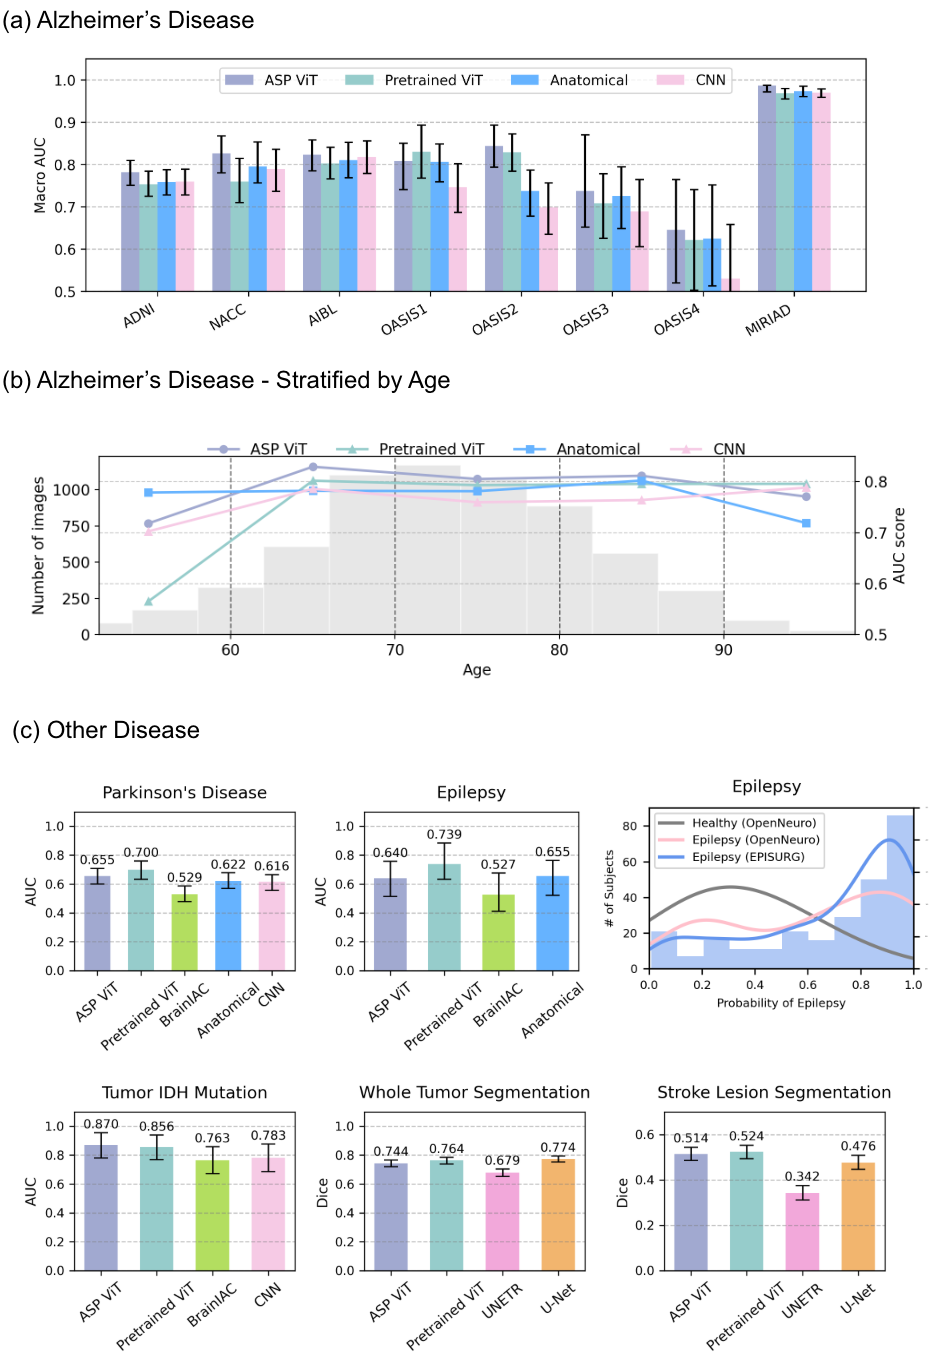
\includegraphics[width=0.95\linewidth,height=0.78\textheight,keepaspectratio]{figures/fig2-dementia-and-disease.png}
\caption{\textbf{Performance comparison across diagnostic and segmentation tasks.} Alzheimer’s disease diagnosis was evaluated across an internal ADNI test cohort and seven external cohorts (NACC, AIBL, MIRIAD, and OASIS 1-4), where ASP ViT achieved the highest macro-AUC in most cohorts, though statistical significance over the CNN and anatomical logistic regression was only reached for OASIS 2. In the diagnostics of Parkinson’s disease (PPMI)\rev{,} \revdel{and Epilepsy (OpenNeuro), }the Pretrained ViT reached the highest AUC, showing a statistically significant improvement only over BrainIAC. \rev{For epilepsy (OpenNeuro), ASP ViT reached the highest AUC, with no statistically significant differences between models.} Estimated probabilities for Epilepsy from ASP ViT are also shown for EPISURG, an additional \rev{external} evaluation set with only epilepsy cases. For the identification of brain tumor IDH mutations (UCSF-PDGM) ASP ViT yielded the highest AUC, though these differences were not statistically significant. CNN could not be applied to the epilepsy task due to limited training data. In segmentation tasks, a U-Net achieved the highest Dice score for adult brain gliomas (BraTS 2023), while the Pretrained ViT performed best for stroke lesion segmentation (ATLAS R2.0); in both cases, the differences were only statistically significant relative to UNETR. Overall, no significant performance differences were observed between the pretrained ViTs, CNNs, and anatomical logistic regression models across the evaluated tasks. \rev{ViT results are obtained with LoRA adaptation (Parkinson's disease and IDH mutation: linear probing). Error bars are 95\% bootstrap confidence intervals; a difference is called statistically significant when the intervals of two models do not overlap.}\revnote{Figure edited: epilepsy ASP ViT bar changed from 0.640 (full finetuning) to 0.751 (LoRA). Its error bar was shifted with the bar and must be replaced with the LoRA confidence interval}
} \label{fig:disease-results}
\end{figure}


\section*{Results}\label{result}

Figure~\ref{fig:overview} provides an overview of the study. We compare the following AI models, adapted to process 3D MRI scans, across different tasks. The models are chosen to represent the main current approaches for image classification and segmentation in data-driven computer vision.   

\begin{itemize}
\item Linear \revdel{logistic-regression }models \rev{(logistic regression for diagnosis, linear regression for brain age)} based on anatomical features consisting of 178 volumes\rev{, surface areas and cortical thicknesses} \revdel{and surfaces }of brain regions (denoted Anatomical in the figures).
\item Convolutional neural networks, which are either ResNets~\citep{he2015deepresiduallearningimage} for classification tasks (denoted CNN) or U-Nets~\citep{ronneberger2015u} for segmentation tasks.
\item Vision-transformer models~\citep{dosovitskiy2020image} pretrained on a large pretraining cohort via masked autoencoding (denoted Pretrained ViT).
\item ViTs pretrained using a novel strategy (Anatomy Segmentation Pretraining, denoted ASP ViT) that leverages anatomical information extracted via segmentation from the scans in the pretraining cohort.
\end{itemize}

The pretraining cohort includes 69,878 MRI scans from 65,249 subjects, primarily from UK Biobank\citep{sudlow2015uk}. More details about the pretraining data are provided in the appendix (Section \ref{sec:pretraining_data}). In addition, we also include comparisons with BrainIAC~\citep{tak2024foundation}, a ViT pretrained using contrastive learning on a different pretraining cohort of 32,000 MRI scans, and UNETR~\citep{hatamizadeh2022unetr}, a medical image segmentation architecture that combines a ViT encoder with a U-Net–style decoder. \rev{The pretrained ViTs are adapted to each task with low-rank adaptation (LoRA), except for the Parkinson's disease and IDH mutation tasks, where linear probing is used (see Methods). All splits are at the participant level, and test and external cohorts were never used for model selection. We report 95\% bootstrap confidence intervals and call a difference statistically significant when the confidence intervals of two models do not overlap, a conservative criterion (see Methods).}     

The models are trained to perform the following seven tasks. The results are shown in Figure~\ref{fig:disease-results}. Additional details about the datasets used to build the training and evaluation cohorts for each task, and the pretraining cohort, are provided in Table~\ref{tab:datasets} and in the appendix (Section \ref{sec:datasets}). 

\begin{itemize}
\item \textbf{Diagnostics of Alzheimer's disease:} The goal is to distinguish between healthy controls, patients with mild cognitive impairment and patients with Alzheimer's disease.
% The training cohort consists of n=4,853 subjects from ADNI~\citep{petersen2010alzheimer}. Evaluation was carried out on an internal test cohort extracted from ADNI (n=1,561), and seven external cohorts, extracted from NACC~\citep{beekly2007national} (n=6,956), AIBL~\citep{ellis2006australian} (n=1,167), MIRIAD~\citep{malone2013miriad} (n=705), and OASIS 1 (n=436), 2 (n=373), 3 (n=2,275) and 4 (n=181) \citep{lamontagne2019oasis,marcus2010open, marcus2007open}. 
The training cohort consists of n=1,453 \revdel{subjects}\rev{participants} from ADNI~\citep{petersen2010alzheimer}. Evaluation was carried out on an internal test cohort extracted from ADNI (n=364\rev{ participants}), and seven external cohorts, extracted from NACC~\citep{beekly2007national} (n=4,926), AIBL~\citep{ellis2006australian} (n=664), MIRIAD~\citep{malone2013miriad} (n=69), and OASIS-1 (n=416), OASIS-2 (n=150), OASIS-3 (n=1,044) and OASIS-4 (n=180)~\citep{lamontagne2019oasis,marcus2010open, marcus2007open}\rev{ (numbers of participants)}.
For the internal test cohort and six external cohorts, ASP ViT has the highest macro-AUC, but the difference with respect to the CNN and the anatomical logistic regression model is only statistically significant for OASIS 2. We didn't apply BrainIAC to this task because its pretraining cohort includes several of our external test cohorts.
\item \textbf{Diagnostics of Parkinson's disease:} The goal is to distinguish between patients with Parkinson's and healthy controls. A training cohort (n=1,572\rev{ scans}) and an internal test cohort (n=460\rev{ scans}) were extracted from PPMI~\citep{marek2011parkinson}\rev{, with no participant in both}. The Pretrained ViT achieves the highest AUC, but the difference is only statistically significant with respect to BrainIAC. 
\item \textbf{Detection of tumor IDH mutations:} The goal is to identify brain tumors with Isocitrate Dehydrogenase (IDH) mutation. A training cohort (n=1,874\rev{ scans}) and an internal test cohort (n=106\rev{ scans}) were extracted from UCSF-PDGM~\citep{calabrese2022university}, which contains labels obtained via genetic sequencing of tissue acquired during biopsy or resection. \rev{Native and contrast-enhanced T1-weighted scans are used as separate single-channel inputs, and predictions are averaged per participant.} ASP ViT achieves the highest AUC, but the difference with the remaining models is not statistically significant. 
\item \textbf{Diagnostics of epilepsy:} The goal is to distinguish between patients with epilepsy and healthy controls. A training cohort (n=82\rev{ participants}) and an internal test cohort (n=81\rev{ participants}) were extracted from OpenNeuro~\citep{schuch2023open}. The models were also applied to Episurg  \citep{perez2021self}, an independent cohort containing only epilepsy cases (n=268). \rev{For an external AUROC, the EPISURG patients were combined with the healthy controls of the OpenNeuro test cohort, none of whom was used for training.} 
%For cross-dataset evaluation, the Episurg  \citep{perez2021self} epilepsy cases (n=268) were evaluated against the healthy-control group from OpenNeuro, since Episurg does not contain healthy controls. 
\revdel{The Pretrained ViT achieves the highest AUC}\rev{ASP ViT achieves the highest AUC (0.751, followed by 0.739 for the Pretrained ViT)}, but the difference with the remaining models is not statistically significant. \rev{On the external evaluation, ASP ViT reaches an AUROC of 0.872 (Supplementary Table~\ref{tab:sc_LoRA_classification}).} We could not apply the CNN to this task due to the limited training data.
\item \textbf{Whole tumor segmentation:} The goal is delineation of adult brain gliomas. A training cohort (n=1,000\rev{ participants}) and an internal test cohort (n=251\rev{ participants}) were extracted from the BraTS 2023 Adult Glioma challenge~\citep{baid2021rsna, menze2014multimodal, bakas2017advancing}\rev{; native and contrast-enhanced T1-weighted scans are used for training and contrast-enhanced scans for evaluation}. The U-Net achieved the highest Dice score (slightly above ASP ViT), but the difference is only statistically significant with respect to UNETR. If the training data is reduced to 10\%, ASP and Pretrained ViT outperform U-Net and UNETR.
 \item \textbf{Segmentation of stroke lesions:} The goal is segmentation of brain lesions associated with stroke. A training cohort (n=355\rev{ scans from 21 acquisition sites}) and an internal test cohort (n=300\rev{ scans from 12 other sites}) were extracted from ATLAS R2.0~\citep{liew2022large}\rev{, so that no site contributes to both}. The Pretrained ViT achieved the highest Dice score (slightly above ASP ViT), but the difference is only statistically significant with respect to UNETR.
\end{itemize}

Overall, we observed that there was no significant difference between the pretrained ViTs, the CNNs and linear models based on anatomical features across the different tasks. \rev{We interpret this as competitive performance under the tested conditions, not as evidence of equivalence: the confidence intervals of the smaller cohorts are wide enough to accommodate moderate differences.} 

\revdel{We conjecture that the inability of the more complex deep-learning models to outperform the simpler linear model is due to the limited training data available for each task. In order to investigate this further,}\rev{A possible explanation for why the more complex deep-learning models do not outperform the simpler linear model is the limited training data available for each diagnostic task. To explore this hypothesis,} we trained the models to estimate \revdel{biological}\rev{brain} age \rev{(i.e., to predict chronological age from the scan of a healthy participant)} using a much larger training cohort drawn from UK Biobank, HCP, CamCAN and IXI (n=62,890\rev{ scans}). Evaluation was carried out on a held-out subcohort from UK Biobank (n=6,950\rev{ scans}), and on two external cohorts of healthy subjects extracted from ADNI (n=2,791) and NACC (n=1,136). \rev{Because this experiment changes both the task and the training-set size, it is consistent with, but does not by itself establish, a sample-size explanation of the diagnostic results.}

Figure~\ref{fig:aging} shows the results on age estimation. The ASP ViT model outperforms the rest, achieving a mean absolute error (MAE) of 2.54 years in the internal test cohort (a) and of 4.19 years in the NACC test cohort (b) and the ADNI test cohort (c). The Pretrained ViT is close in performance on the internal test cohort (0.35 years greater), but the gap widens for the external cohorts (more than 1 year greater). The \revdel{logistic}\rev{anatomical linear} regression model performs worse than the ViT approaches by a significant margin (between 1 and 2 years), but clearly outperforms the CNN. \rev{The ranking is the same in the internal and both external cohorts, and on every metric (mean absolute error, mean squared error and Pearson correlation; Supplementary Table~\ref{tab:healthy_aging_results}).} The performance differences are maintained when stratifying the data by sex. Stratifying by age reveals that the differences between the models are mainly driven by the superior performance of the ViT models (particularly ASP ViT) on subjects with advanced ages (above 80), which are less represented in the training and pretraining cohorts, especially with respect to the CNN. \rev{As is common for brain-age models, predictions are biased towards the mean age of the training cohort, which explains the larger errors above 80 years (Figure~\ref{fig:aging}); no post-hoc bias correction was applied, so all models are compared on their raw predictions.} 

The best-performing age-estimation model was also applied to mildly-cognitively impaired (MCI) and dementia patients from the NACC and ADNI  datasets, as shown in Figure~\ref{fig:aging}(b,c). Age estimates for dementia patients were consistently above their \revdel{biological}\rev{chronological} age, in most age intervals for both cohorts. The effect also exists to some extent for MCI subjects, but is less pronounced. \rev{These group-level differences are consistent with accelerated brain atrophy in neurodegeneration; they are reported as supporting evidence, and establishing the clinical value of these estimates would require dedicated outcome studies.}


\begin{figure}[tp!]%
\centering
  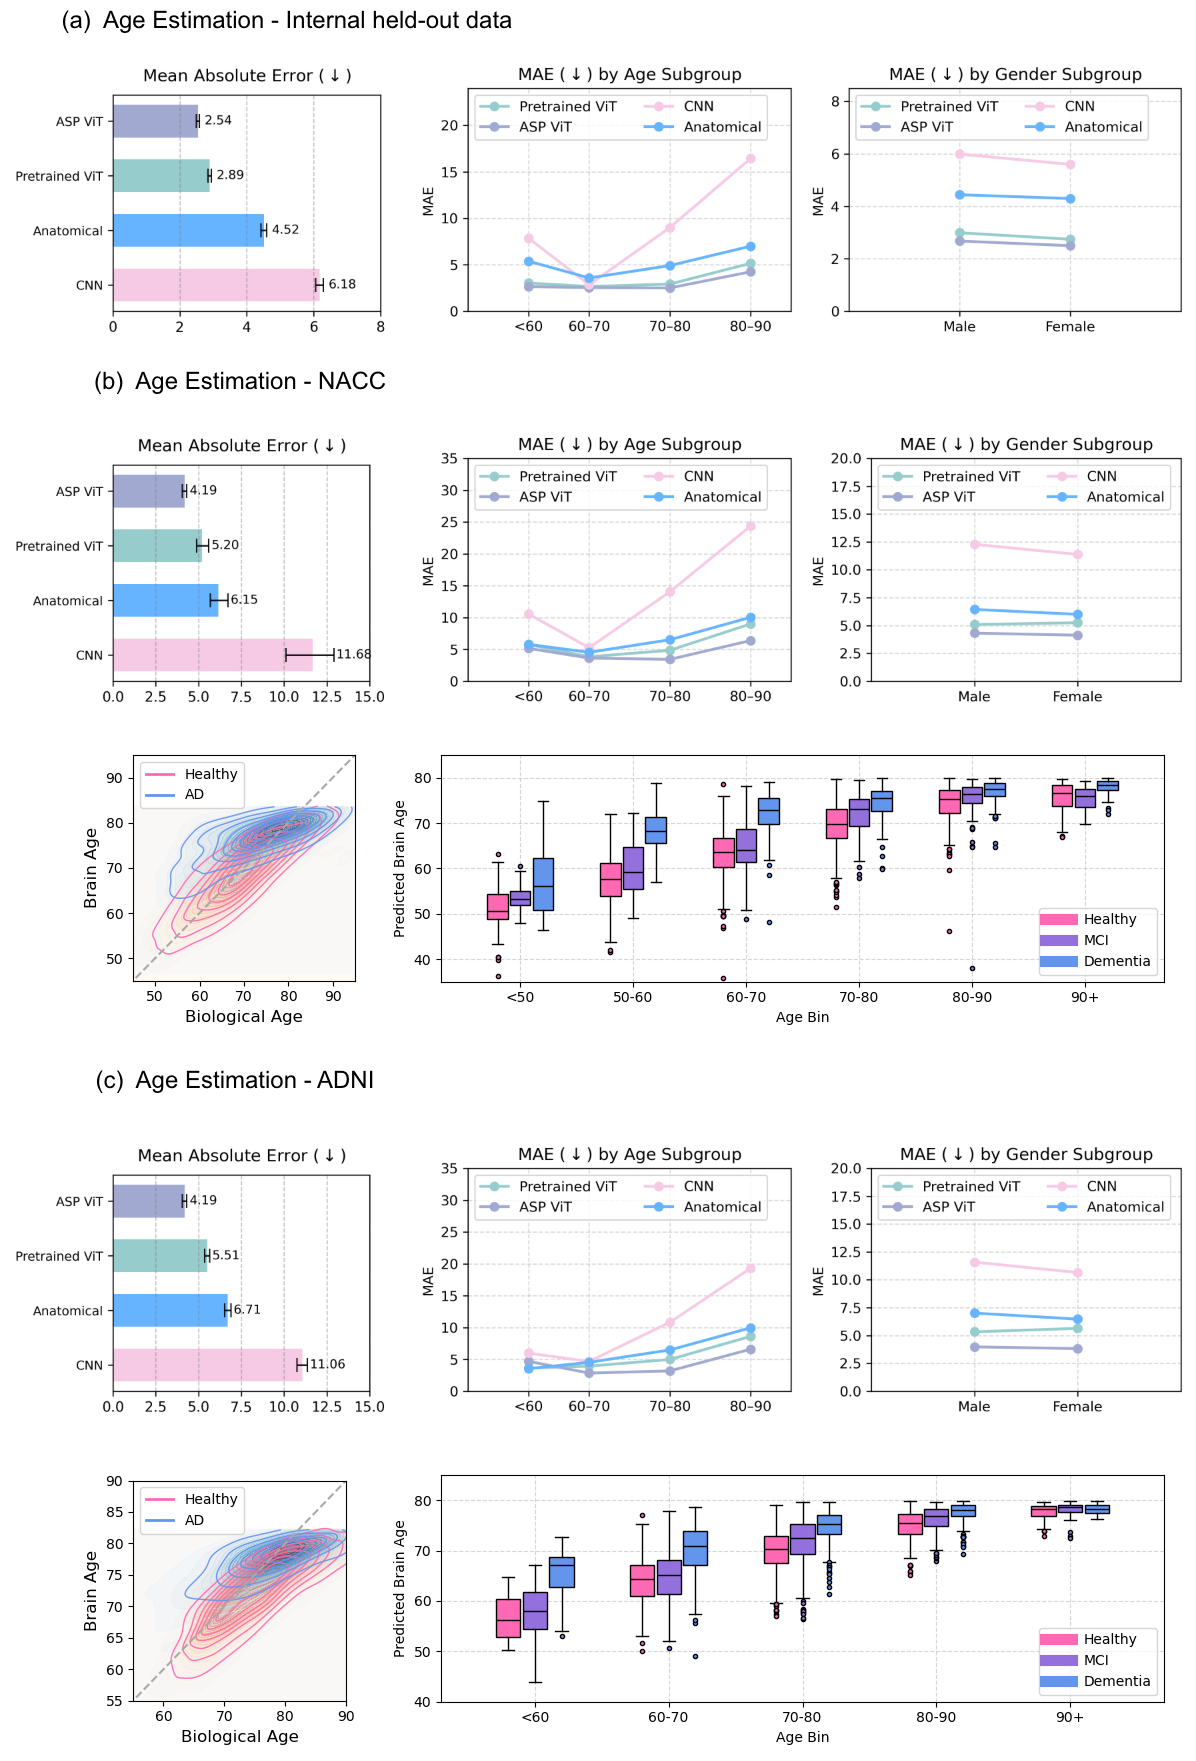
\includegraphics[width=0.95\linewidth,height=0.79\textheight,keepaspectratio]{figures/fig3-Age-result.png}
\caption{\textbf{\rev{Brain} age estimation performance across internal and external cohorts.} The ASP ViT model demonstrates superior performance, achieving a mean absolute error (MAE) of 2.54 years in the internal test cohort (a) and 4.19 years in both the NACC (b) and ADNI (c) external test cohorts. While the Pretrained ViT maintains competitive performance on the internal cohort with an MAE only 0.35 years greater than the ASP ViT, this performance gap widens to over 1 year in the external cohorts. \revdel{Logistic}\rev{The anatomical linear} regression \rev{model} underperforms relative to the ViT-based approaches by a margin of 1 to 2 years, though it consistently outperforms the CNN. These performance comparisons remain stable when the data is stratified by sex and age. Age-based stratification reveals more pronounced errors for individuals over 80, a demographic less represented in the training and pretraining datasets. When the best-performing model (ASP ViT) is applied to clinical populations, age estimates for dementia patients from the NACC (b) and ADNI (c) datasets are consistently higher than their \revdel{biological}\rev{chronological} age across most age intervals.
} \label{fig:aging}
\end{figure}

% 

% In the remainder of this section, we provide more details about each task and report the results.


% \subsection*{Alzheimer's Disease}

% The task was to distinguish between patients with Alzheimer's disease, patients with mild cognitive impairment (MCI), and healthy controls. 

% We compared a linear model based on anatomical features (XXX volumes and surfaces extracted using Freesurfer), a CNN trained on, and two ViT models pretrained on... and finetuned on... One ViT model is pretrained using MAE, the other... 

% We used ADNI\citep{petersen2010alzheimer} as a training dataset and evaluated on 7 independent test sets: NACC\citep{beekly2007national}, ADNII\citep{petersen2010alzheimer}, AIBL\citep{ellis2006australian}, OASIS1\citep{lamontagne2019oasis,marcus2010open, marcus2007open}, OASIS2, OASIS3, OASIS4 and MIRIAD\citep{malone2013miriad}. 

% Evaluation metric was macro AUC. All models performed similarly...

% \subsection*{Parkinson's Disease}

% We use PPMI\citep{marek2011parkinson} for developing and validating a model trained for PD diagnosis at the time of scan. Given the longitudinal nature of PPMI, we split the dataset in a subject-wise way to avoid data leakage. We use 20\% of the PPMI participants data (n=460) as a held-out test cohort for assessing model performance.

% \subsection*{Tumor IDH Mutation} 

% We use UCSF-PDGM\citep{calabrese2022university} to investigate imaging markers for Isocitrate dehydrogenase (IDH) mutation. All subjects’ tumors were tested for IDH mutations by genetic sequencing of tissue acquired during biopsy or resection. We use any IDH mutation versus no mutation (“Wildtype”) as our task of interest. We split the data subject-wise, leaving 20\% (n=106) subjects as our held-out test cohort. The rest of the data is used for adapting the foundation model. All T1 and T1 with contrast enhancement images are included in this task. During training, we optimize for mutation label for each image. During evaluation, we aggregate model predicted probability for IDH mutation or each subject.

% \subsection*{Epilepsy}

% We use OpenNeuro\citep{schuch2023open} dataset to develop a model that identifies FCD caused by epilepsy. Since this is a rather smaller dataset compared to other tasks, we randomly split 50\% the dataset by  to have n=82 subjects as our held-out test cohort.

% \subsection*{Tumor Segmentation}

% We include T1 MRI scans from BraTS 2023 Adult Glioma challenge training cohort\citep{baid2021rsna, menze2014multimodal, bakas2017advancing}. Each subject received two T1 scans, one with contrast enhancing(CE) agent, one without. All the imaging datasets have been annotated manually by experienced neuro-radiologists. No coregistration is applied to this dataset so that we can compare the original manual segmentations without the complication of interpolating segmentation masks. We first split the subjects into training (n=1000) and testing (n=251) cohort using subject-wise random split. To simulate the few-shot learning use case, we further randomly sample two small subsets of the training subjects (n=100, n=300) to train the segmentation model. To make best use of all T1 images, we train models regardless of using contrast enhancing (CE) agent or not, and evaluate the models using predictions on T1 with CE.


% \subsection*{Stroke Lesion Segmentation}

% We use ATLAS R2.0\citep{liew2022large} to study stroke lesion segmentation task. No further coregistration is applied to this dataset, as the images are already coregistered to the same template used in our study. There are 655 scans from 33 subjects in the dataset. Some subjects receive far more repeated scans than others. For instance, there are 111 scans from subject r009, but only 2 scans from subject r044. To mitigate this imbalance in scan numbers across subjects, we only include subjects with 10\~50 scans in the test cohort. We randomly select 12 subjects to form the test set with 305 scans, the remaining 355 scans from 21 subjects comprise the training set. Notably, this is a very challenging task with a small training set, we do not further downsample the training data.


% \subsection*{Brain Aging}

% As UKBB\citep{sudlow2015uk} is a general population, we explicitly excluded 274 participants with lifetime brain diseases, including diseases linked to the central nervous system (ICD-10 code: G group in Data-Field=41202, 41204, 41270 or with dementia reported dates in Data-Field=130836, 130838, 130840, 130842) and neurocognitive disorders (ICD-10 code: F in Data-Field=41202, 41204, 41270). We combine the identified healthy participants in UKBB with all subjects from HCP, CamCAN, IXI to arrive at a healthy aging training cohort. We use 10\% of the participants for model validation to monitor the pretraining process. We then evaluate the trained model to healthy subjects in ADNI and NACC to assess the robustness of our healthy brain age model. We further investigate the predicted age’s correlation with dementia risk using ADNI\citep{petersen2010alzheimer} and NACC\citep{beekly2007national}.


%MRI-based brain age prediction is associated with neurocognitive function~\citep{marin2024brain, lee2022deep, biondo2022brain} in aging adults and may have utility as an early biomarker for Alzheimer’s disease. To evaluate NeuroVision as a foundation for improved brain age prediction, we full finetune the model to predict biological age on healthy pretraining subjects (n=62,000). We reserve a held-out cohort of 6950 healthy people from pretraining subject as internal validation. In addition, we use 2791 T1 images from NACC healthy subjects as our external cohort. We only include external participants who are less than 90 years old to match the age range in the healthy aging adaptation population. Performance was assessed using Mean Absolute Error (MAE) and Pearson Correlation (CORR) for predicted age versus biological age. 

%In our experiments, we observe that training neural networks from scratch on structural MRI (CNN) yields limited generalization to unseen external cohorts drawn from different datasets. In contrast, simple models leveraging brain anatomical statistics (LR\_Anat) demonstrate stronger predictive performance, underscoring that the underlying task is non-trivial and requires informative priors to be effectively learned. These findings highlight the need for robust pretraining strategies to capture relevant structural features before downstream model adaptation. Our proposed method, AGPT, regradless of LoRA or full fintunine, consistently achieves the best performance across all evaluated age groups, as in \ref{fig:aging-result},  producing the lowest prediction error and demonstrating strong generalizability.

%Finally, we assess whether the predicted brain age provides clinically meaningful signals in dementia populations. As shown in \ref{fig:aging-result}, we find that individuals with dementia exhibit significantly elevated predicted brain age relative to their chronological age, suggesting accelerated structural aging and supporting the potential utility of our model as a biomarker of neurodegenerative abnormality.

%Structural Brain MRI images are particularly useful for detecting atrophy (shrinkage) of specific brain regions, which is a hallmark of various types of dementia, including Alzheimer's disease (AD) and Frontotemporal Dementia (FTD). We gather multiple dementia related neuroimaging datasets: NACC, ADNI, AIBL, OASIS1, OASIS2, OASIS3, OASIS4 and MIRIAD, with \textcolor{red}{18985} images to investigate the performance for dementia related tasks. We focus on discriminating among three clinically relevant categories: Dementia, Mild Cognitive Impairment (MCI), and Healthy Control (HC). We applied AGPT pretrined model to a subset of ADNI to adapt to the task of dementia detection and povided test performances in Fig \ref{fig:dementia-result}.

% Given that dementia is a progressive condition in which patients typically transition through an intermediate MCI stage prior to formal dementia diagnosis, we design a loss function that explicitly reflects this ordinal structure. Instead of treating the problem as a standard three-class classification task, we assign soft labels—0 for HC, 0.5 for MCI, and 1 for Dementia—and optimize the model using a binary cross-entropy objective. This formulation captures the continuum of disease severity and yields superior performance compared to conventional multiclass classification approaches (results shown in the Appendix \ref{sec:preliminary_analysis}).

%Consistent with our findings in the brain age prediction task, anatomical features again outperform models trained directly on raw MRI images, highlighting the importance of structural priors in neurodegeneration-related tasks. Our proposed Anatomy-Guided Pre-Training (AGPT) method achieves the strongest overall performance across all evaluation settings. Subgroup analyses further demonstrate that AGPT maintains robust improvements across demographic and clinical subsets, underscoring its generalizability and effectiveness for dementia detection.


% And other things we've tried to get to this method, such as iterative learning, frozen decoder, etc.

% Base pretraining methods comparison, MAE vs DINO.

% Adaptation methods, a comparison between LoRA and Full Finetune. 

% LoRA implementation details, hyper parameter choice and lessons learnt from it.


%\clearpage

\section*{Discussion}\label{discussion}

Our study demonstrates that across a wide range of publicly available structural MRI datasets, linear models trained on preselected anatomical features remain highly competitive with deep neural networks. While traditional segmentation approaches are often computationally expensive for feature extraction, modern deep learning-based segmentation frameworks (e.g., FastSurfer \citep{henschel2020fastsurfer}) offer an efficient alternative. Our results suggest that leveraging these deep-learning tools to extract structured anatomical features for linear models provides a computationally efficient, interpretable, and robust baseline for various diagnostic tasks. \rev{Two aspects of the study design support this conclusion. All models were compared on the same participant-level splits, and on external cohorts that were never used for training or model selection. In addition, the anatomical models are linear and use a fixed, predefined feature set, so their external performance cannot be explained by tuning to the evaluation cohorts. The compared pipelines differ in more than the representation alone (for instance in preprocessing and training procedure); our comparison therefore characterizes complete pipelines as they are used in practice, rather than isolating a single factor.}

Furthermore, our results indicate that diagnostic performance using structural MRI \revdel{may have reached a saturation point within}\rev{is currently limited less by the choice of model than by the size of} existing public datasets\rev{, which} \revdel{that }contain only hundreds to a few thousand scans \rev{per task}. Further progress will likely require the curation of substantially larger cohorts. Our age-estimation experiments on a cohort of \revdel{60,000 subjects}\rev{more than 60,000 scans, where the pretrained ViTs clearly outperform both the anatomical model and the CNN,} indicate that scaling public datasets could unlock further methodological innovation. 

From the methodological perspective, we show that vision transformers learn relevant anatomical structure during unsupervised pretraining, but at a slow rate that can be \revdel{greatly }accelerated using anatomical segmentation as an auxiliary pretraining task. \rev{ASP ViT achieved the best result in five of the seven tasks (Alzheimer's disease, IDH mutation, epilepsy and age estimation in all three cohorts), with the clearest gains in age estimation on the external cohorts, where it reduced the error of the Pretrained ViT by more than one year. The ablation study (Figure~\ref{fig:ASP}(e)) shows that these gains come from the complete ASP procedure: initializing from MAE, training the decoder on the frozen encoder, and alternating segmentation with MAE updates each contribute to the final performance. Because the segmentation decoder is discarded after pretraining, the anatomy-informed encoder has the architecture and inference cost of a standard ViT and can be used as a drop-in replacement in existing pipelines.} This suggests that leveraging clinically-relevant tasks could mitigate the small size of medical pretraining datasets when compared to general computer-vision pretraining databases with millions of examples. 

\rev{\textbf{Limitations.} Our study has several limitations. First, we used T1-weighted structural MRI only; other sequences such as FLAIR or diffusion MRI may carry complementary information, particularly for tumors, stroke lesions and epilepsy. Second, several downstream cohorts are small (for example, 82 training participants for epilepsy), which widens the confidence intervals and limits the power to detect moderate differences between models. Third, ASP adds pretraining epochs on top of MAE; although MAE pretraining had converged before ASP started, we did not train a compute-matched MAE baseline. Fourth, as is common for brain-age models, age estimates are biased towards the mean of the training cohort, and we did not apply post-hoc bias correction. Fifth, the anatomical labels used for ASP and the anatomical features are produced automatically by FreeSurfer and are therefore imperfect, especially for small structures. Finally, public research cohorts are not fully representative of clinical populations in terms of demographics, scanners and disease severity, so performance in routine clinical settings remains to be established. Addressing these points, for instance with multi-sequence pretraining and larger disease cohorts, is a natural next step that the released code and models are designed to support.}


\section*{Methods}\label{sec:method}

In this section, we first present a new technique for pretraining vision transformers (ViTs) using anatomical information. Then, we describe the remaining methodology in our study, including masked autoencoder pretraining of ViTs, downstream application of pretrained ViTs, linear models based on anatomical features, convolutional neural networks, and data preprocessing.

\subsection*{Anatomy Segmentation Pretraining of Vision Transformer}

We propose a novel approach to pretrain ViTs on MRI data. The goal is to inject anatomical information into the model during pretraining. The motivation is that simple models that rely only on anatomical information, such as the \revdel{logistic-regression model}\rev{linear models} with brain-region volume\rev{, surface-area and thickness} \revdel{and surface }features used in this study, can be very effective (see Results section). 

We build upon a key observation: when pretraining ViTs via masked autoencoding (MAE), the model automatically learns embeddings that reflect anatomical information, but only to some extent. The green region in the graph from Figure \ref{fig:ASP}(b) shows the accuracy of predicting the volumes of different brain regions from MAE embeddings via linear probing during training. The accuracy increases, indicating that the embeddings gradually capture anatomical information. In order to further boost the anatomical information learned by the model, we propose to incorporate brain-region segmentation as an auxiliary task during pretraining. 

Our procedure to perform anatomy segmentation pretraining (ASP) is illustrated in Figure \ref{fig:ASP}(a). A 3D ViT produces the embedding used for downstream tasks. After MAE pretraining (green region in Figure \ref{fig:ASP}(b)), we train a lightweight mask decoder to perform segmentation of different brain regions in two phases. First, the ViT parameters are frozen\rev{ for 100 epochs} to ensure that the decoder learns how to use the existing embedding for segmentation (yellow region in Figure \ref{fig:ASP}(b)). Next, the encoder and decoder are trained jointly. In this ASP phase, segmentation and MAE pretraining are performed in alternating epochs\rev{ (one segmentation epoch followed by one MAE epoch)} to prevent the model from \textit{forgetting} useful features learned via MAE. This strategy is common in continual-learning methods that balance new-task adaptation with the retention of prior knowledge \cite{Kirkpatrick2017,li2017,rebuffi2017}.

Regions for ASP were selected based on their disease relevance and anatomical scale. We discarded regions that lacked a strong disease association and contributed less than 1\% of the total brain volume. To further improve efficiency, symmetrical structures (such as the left and right hippocampus) and anatomically related sub-units (such as segments of the corpus callosum) were consolidated into single labels. This resulted in 39 distinct regions, listed in Figure \ref{fig:ASP}(c). More details are provided in \revdel{the Appendix}\rev{Supplementary} Section \ref{sec:anatomical_segmentation_workflow}.
%Starting from a pretrained encoder, we continue training it using brain region segmentation as supervision. The goal is to adapt the [CLS] token so that it encodes not only the general visual features learned during pretraining but also anatomically relevant structure. Implementing this required addressing several practical challenges along the way.

The segmentation architecture used to perform ASP is tailored specifically to the pretraining task. Deep-learning segmentation models typically rely heavily on skip connections, which emphasize local feature fusion and reduce the importance of global representations ~\cite{ronneberger2015u}, ~\cite{hatamizadeh2022unetr}. In contrast, the goal of ASP is to concentrate the anatomical information in the ViT embedding. To address this, we use a bottleneck decoder architecture(see Figure \ref{fig:seg_decoder}), where the segmentation prediction is generated directly from the ViT embedding, without any skip connections. The decoder is lightweight, in order to further encourage the model to concentrate rich anatomical information in the ViT transformer. More details are provided in \revdel{the Appendix}\rev{Supplementary} Section \ref{sec:seg_architecture}.

A key challenge is applying ASP to a relatively large number of anatomical regions (39, as explained above). A naive implementation based on a standard softmax output would be too memory intensive, as it would require generating 39 different 3D logit maps (39×128×128×128). Instead, we adopt a prompt-based architecture, inspired by \cite{liu2024uncertainty}, where a prompt is used to adapt the Segment Anything Model~\cite{kirillov2023segment} to different segmentation tasks. A \textit{brain-region prompt} indicates which brain region should be segmented by the lightweight decoder, and the decoder output is compared to a binary segmentation task indicating the appropriate region (see Figure \ref{fig:ASP}(a)). The brain region is selected at random during pretraining. 

We trained the ASP model for 400 epochs with a batch size of 16 per GPU. We used binary cross entropy and the AdamW optimizer ($\beta_{1} = 0.9$, $\beta_{2} = 0.95$, weight decay = 0.04), with a base learning rate of $5\times10^{-4}$. We applied learning rate scheduling via cosine annealing with linear warm-up over the first 5 epochs. Convergence is observed at around 200 epochs, requiring approximately one month of training on a single \revdel{42GB NVIDIA RTX8000}\rev{48GB NVIDIA Quadro RTX 8000} GPU. \rev{ASP starts from the MAE checkpoint, whose pretraining had already converged at around 900 of its 1000 epochs (see below); the additional MAE epochs performed during the alternating phase are therefore unlikely to explain on their own the differences between ASP ViT and the Pretrained ViT. The segmentation decoder and the region prompts are used only during pretraining and are discarded afterwards, so ASP ViT has exactly the same architecture, number of parameters and inference cost as the Pretrained ViT.}

Figure \ref{fig:ASP}(c) reports the performance of the decoder for the different regions before and after the ASP phase, showcasing that the model is indeed able to learn how to segment the different regions reasonably accurately (although its performance for smaller or more intricate region is relatively modest). Figure \ref{fig:ASP}(d) shows some examples of segmentation outputs, compared to the ground truth. Figure \ref{fig:ASP}(e) provides an ablation study, which establishes that each element in the proposed framework (prior MAE pretraining, initial freezing of the encoder to train the decoder, and alternating with MAE to avoid forgetting) all provide a non-negligible increase in performance for the downstream task of age estimation. Further information about the ablation study is provided in \rev{Supplementary Section~}\ref{ablation_study}.

% \begin{enumerate}[label=\roman*.]
%   \item \textbf{Integrating anatomical information into the [CLS] token:} Conventional 3D segmentation pipelines are not directly applicable in this context. The ultimate goal of widely used segmentation architectures (e.g., UNet, SwinUNETR) is to provide a whole architecture able to segment. However the goal of this segmentation pre-training stage is to add information to the [CLS] token. These architectures rely heavily on skip connections, which emphasize local feature fusion and reduce the importance of global representations ~\cite{ronneberger2015u}, ~\cite{hatamizadeh2022unetr}. This contradicts our aim of centralizing anatomical representation in the [CLS] token.
  
%   To address this, we introduced a bottleneck decoder architecture, where the segmentation prediction is generated directly from the [CLS] token without any skip connections with a simple decoder. This enforces a learning signal that flows solely through the global embedding, encouraging it to encode as much anatomical detail as possible. Selecting a small, plain mask decoder (see Figure ~\ref{fig:seg_decoder}) keeps most of the model’s capacity in the ViT encoder. Because the head cannot add much detail on its own, the image embedding is forced to preserve rich anatomical information. This design choice effectively mitigates the issue of global feature dilution.
%   \item \textbf{Memory limitations due to multi-label 3D segmentation:} Standard 3D segmentation pipelines cannot be used directly in this context due to the memory-intensive nature of 3D label volumes. For example, label maps for all 39 anatomical regions span dimensions of 39×128×128×128, making it impractical to use them with reasonable batch sizes in GPU memory.
  
% Instead of training the model to segment all 39 anatomical regions simultaneously, we adopt a region-wise, prompt-based training strategy, inspired by prompt learning approaches such as those used in SAM~\cite{kirillov2023segment}. In this approach, the model focuses on predicting a single region per forward pass, which reduces the supervision target to a binary mask of size $2 \times 128 \times 128 \times 128$. Each forward step is guided by an external region identifier, provided in the form of a learned prompt vector retrieved from a prompt embedding matrix. This matrix acts as a lookup table, where each anatomical region is associated with a dedicated trainable embedding (see Figure ~\ref{fig:emb_matrix}). These embeddings condition the model to attend to the specific region of interest, enabling a lightweight mask decoder to output only one region mask at a time. The whole architecture of the prompt-based encoder can be seen in Figure ~\ref{fig:prompt_arch}. Furthermore, by iterating over all regions across training steps, the model’s shared [CLS] token becomes exposed to diverse anatomical structures, progressively learning to encode region-specific representations in a generalizable way. This strategy greatly reduces memory consumption, allowing for larger batch sizes and more stable training dynamics.


% \item \textbf{Risk of catastrophic forgetting:} Sequentially optimizing a model for different objectives—first through self-supervised learning and later through supervised segmentation—often leads to catastrophic forgetting, where the network adapts to the new task at the expense of previously learned representations \cite{Kirkpatrick2017,li2017,rebuffi2017}. In our case, training the ViT encoder to predict anatomical segmentations risks overwriting the general visual features acquired during MAE pretraining.

% To reduce this effect, we adopt a two-stage and alternating training strategy. First, we freeze the pretrained encoder for 100 epochs while training only the segmentation components (decoder and region prompt embeddings), ensuring they adapt to the existing MAE features rather than forcing the encoder to change prematurely. After this warm-up phase, we alternate between one epoch of MAE pretraining and one epoch of supervised segmentation. This interleaving helps preserve the encoder's general visual representations while still enabling it to incorporate anatomically relevant information. This approach follows the principle used in well-established continual-learning methods that balance new-task adaptation with the retention of prior knowledge \cite{Kirkpatrick2017,li2017,rebuffi2017}.
%  segmentation task.
% \end{enumerate}\\

% Training is conducted as follows: the image dataloader operates conventionally, loading full 3D MRI volumes. However, for each input image, a corresponding label is generated by randomly selecting one brain region index and retrieving its binary mask along with the associated region prompt. To promote exposure to diverse anatomical targets and reduce overfitting, the label dataloader is regenerated at the start of each epoch, ensuring that different region targets are sampled throughout training.\\
% \\
% We train the segmentation model for 400 epochs with a batch size of 16 per GPU. We used the BCE(Binary Cross Entropy) loss as the objective. The optimizer is AdamW ($\beta_{1} = 0.9$, $\beta_{2} = 0.95$, weight decay = 0.04), with a base learning rate of $5\times10^{-4}$. Learning rate scheduling uses cosine annealing with linear warm-up over the first 5 epochs. When using 100\% of the data, convergence is observed at around 200 epochs, requiring approximately one month of training on a single 42GB NVIDIA RTX8000 GPU.\\


\begin{figure}[h]
  \centering
  \includegraphics[width=1\linewidth]{figures/seg_mae.png}
\caption{\textbf{a. Prompt-based segmentation architecture}. The input consists of an image and a brain region index, which is used to retrieve the corresponding brain region embedding. This embedding is added to the image representation, and the combined features are passed through a lightweight decoder to predict the segmentation mask for the specified region. \textbf{b. Linear‑probe accuracy/$R^{2}$} on six target variables—two global attributes (age, gender) and four region‑specific volumetric measures—tracked over pre‑training epochs. The differences in overall accuracy across regions arise because some regions are inherently easier to predict than others. For example, cortex volume tends to be more accurately segmented due to its larger size and higher contrast, compared to smaller and less distinct regions like the hippocampus. For demographic statistics the same happens. Gender is easier to infer than age since it is a binary attribute, while age requires finer-grained regression. \textbf{c–d. Validation IoU by Brain Region.} Regional performance varies based on anatomical complexity; for instance, the superior frontal cortex's small, irregular geometry results in lower IoU, whereas the smoother, more consistent morphology of the pallidum allows for higher segmentation accuracy. \textbf{e. ASP training ablation.} Age-estimation performance for different ASP training variants on the external NACC cohort. The full ASP model achieves the lowest error, while removing alternating MAE updates, removing encoder freezing, using MAE alone, or training from scratch reduces performance. Detailed results are provided in Appendix Section~\ref{ablation_study}.}
  \label{fig:ASP}
\end{figure}



\subsection*{Masked Autoencoder Pretraining of ViTs}

Masked Autoencoding (MAE) is a self-supervised learning framework that trains ViTs by reconstructing masked images, which are missing a random subset of their pixels~\citep{he2022masked}. We adapted this framework to process 3D structural MRI volumes. We used a ViT-Base encoder adapted to 3D inputs, consisting of 12 transformer blocks with 12 attention heads and a 768-dimensional embedding, using 16×16×16-voxel patches. During pretraining, 75\% of the 3D patches in each volume were randomly masked, and the ViT was trained to reconstruct the original volumes from the unmasked patches. Volumes were represented as single-channel inputs with intensities scaled to $[0,1]$; images were padded to $256 \times 256 \times 256$, randomly cropped to $128 \times 128 \times 128$, and augmented with random flipping and intensity shifting. Pretraining used mean squared error (MSE) reconstruction loss for 1000 epochs with batch size 32 per GPU, AdamW~\citep{loshchilov2017decoupled} ($\beta_1=0.9$, $\beta_2=0.95$, weight decay $=0.005$), and a cosine learning rate schedule~\citep{loshchilov2016sgdr} with base learning rate 0.0015 and linear warm-up during the first 2.5\% of training steps.  Convergence is observed at around 900 epochs, which took around 10 days on two 80GB NVIDIA A100 GPUs.


\subsection*{Downstream Application of Pretrained ViTs}

To adapt the pretrained ViTs for downstream applications, we feed the resulting embeddings into task-specific output modules: a binary-classification head for diagnostic tasks, a linear-regression head for regression tasks (e.g. estimation of age or of anatomical features) and a U-Net–style decoder for voxel-level segmentation, following the UNETR architecture~\citep{hatamizadeh2022unetr}. See Section \ref{sec:mae_additional} for additional details. The pretrained ViTs were adapted to the different downstream tasks using the following strategies. 

\begin{itemize}
\item \textbf{Linear probing:} The linear regression and classification heads were trained to generate predictions from the ViT embedding, using the \texttt{sklearn} implementations of logistic regression and ordinary least squares. This approach was used as a diagnostic tool during pretraining to monitor representation quality using anatomical and demographic targets, as illustrated by Figure \ref{fig:ASP}(b). It was also used for diagnostics of Parkinson's disease and detection of tumor IDH Mutation, due to the small size of the training datasets.

% \item \textbf{Full finetuning:} The entire ViT encoder was finetuned jointly with task-specific heads. We employed random cropping for regularization during training and at inference time we used center crop for classification tasks and a sliding window approach for full-volume segmentation tasks. Training was performed with the AdamW optimizer for 150 epochs. This was applied to all remaning tasks. In the case of the epilepsy diagnostics task, we applied partial finetuning, updating only the final attention block for 60 epochs. 

\item \textbf{Low-Rank Adaptation (LoRA):} Both ViT encoders (ASP and pretrained) were adapted using LoRA ~\citep{zhu2024melo, hu2022lora}: the original model parameters were kept frozen, and trainable low-rank matrices were introduced into the attention layers. These low-rank parameters were optimized jointly with the task-specific heads, substantially reducing the number of trainable parameters compared with updating the entire encoder. \rev{LoRA was applied to the query, key and value projections of every transformer block. All ViT results reported in the main text were obtained with LoRA, except for Parkinson's disease and IDH mutation, where linear probing was used.} Random cropping was employed for regularization during training. At inference time, we used center cropping for classification tasks and a sliding window approach for full-volume segmentation tasks. Training was performed with the AdamW optimizer for 150 epochs. 

\item \textbf{Full Finetuning:} \revdel{For ablation experiments,}\rev{As an alternative adaptation strategy,} we updated all parameters from the ASP ViT encoder jointly with the downstream head using the same optimization and augmentation settings as LoRA. \rev{The resulting performance is reported in} \revdel{See Appendix}\rev{Supplementary} Section \ref{sec:additional_model_training_details}.

\end{itemize}

\rev{\textbf{Data splits and model selection.} All training, validation and test splits were defined at the participant level, so that scans of the same participant never appear in more than one split. None of the disease cohorts used for downstream evaluation is part of the pretraining cohort, and the UKBB participants of the internal age-estimation test cohort were excluded from MAE and ASP optimization. For every model, hyperparameters and checkpoints were selected on validation data taken from the training cohort of each task (e.g., early stopping on validation loss); internal test sets and external cohorts were used only for the final evaluation. The UKBB holdout was used to monitor representation quality during pretraining (Figure~\ref{fig:ASP}(b)) but not to select models or checkpoints.}

%For downstream tasks, the pretrained encoder was adapted using two complementary strategies: linear probing and finetuning. In all cases, input volumes were padded to \(256\times256\times256\), and \(128\times128\times128\) 3D crops were used as input to the ViT. For image-level tasks, predictions were obtained by attaching a task-specific linear head to the CLS token. Additional implementation details and are provided in the Appendix Section~\ref{sec:mae_additional}. For dense prediction tasks, namely stroke lesion and whole-tumor segmentation, the pretrained ViT encoder was combined with a U-Net–style decoder that upsamples the encoder features and predicts a class label for each voxel.

% \begin{itemize}
% \item \textbf{Linear probing. } 

% \end{itemize}

% \subsubsection*{Linear Probing}

% In the linear probing setting, the pretrained ViT backbone was kept frozen and only a linear prediction head was trained on top of the learned representation. We used the central crop of each MRI volume in order to provide a stable and consistent view of the anatomy, and optimized only the parameters of the classifier or regressor. 

% For Parkinson's Disease and Tumor IDH Mutation results in Figure \ref{fig:disease-results}, we applied linear probing to ASP ViT and Pretrained ViT to get predictions. In practice, it was particularly useful with small datasets and scenarios where we wanted to directly assess the transferability of the learned representation to downstream clinical discrimination. It also provides a clean comparison against supervised baselines and anatomical-feature models. We used the standard Logistic Regression implementation in sklearn library with liblinear solver and max\_iter=1000 on top of extracted embeddings to get predictions for each scan. 

% For monitoring in-training representation quality, we also applied linear probing on extracted embeddings during pretraining. The targets were not disease labels but rather volumetric measures of the brain regions and global attributes (age, gender). This setting was used to evaluate how much disease-relevant information was already encoded in the pretrained features. We applied plain Ordinary Least Squares Linear Regression for volumetric measures and age, and same Logistic Regression setup for gender as above, both using sklearn library.

% \subsubsection*{Full-Finetuning}

% In the full-finetuning setting, the entire pretrained encoder was updated jointly with a task-specific head, allowing the representation to specialize to the downstream objective. We applied full finetuning for segmentation tasks, where we adopted UNETR~\citep{hatamizadeh2022unetr} architecture with a U-shape decoder, taking learned brain structural representation and raw image, then generating segmentation masks. During training, we used random crops for regularization, while a sliding window approach for entire 3D image was used at validation and test time. We used the same optimizer and early stop method as in the linear probing diagnostic disease prediction case. In low-data regimes, we also explored partial finetuning, updating only the last attention block, which was especially useful for epilepsy to reduce overfitting while still adapting the pretrained features,as show in Figure \ref{fig:disease-results}. Overall, these adaptation strategies let us balance transferability and specialization depending on the difficulty and size of each downstream task. We inherited the AdamW optimizer and early stopping setup from MAE Pretraining and trained 60 epoch for epilepsy and 150 epochs for segmentation.

% % During training, we used random crops for regularization, while the central crop was used at validation and test time. This strategy was preferred for tasks that benefit from stronger adaptation to subtle disease-specific morphology or from larger amounts of labeled data, such as dementia-related prediction tasks, including Alzheimer’s disease diagnosis, as well as healthy brain aging estimation. In low-data regimes, we also explored partial finetuning, updating only the last attention block, which was especially useful for epilepsy to reduce overfitting while still adapting the pretrained features. Overall, these adaptation strategies let us balance transferability and specialization depending on the difficulty and size of each downstream task.

% \subsubsection*{LoRA}


% During training, we used random crops for regularization, while the central crop was used at validation and test time. This strategy was preferred for tasks that benefit from stronger adaptation to subtle disease-specific morphology or from larger amounts of labeled data, such as dementia-related prediction tasks, including Alzheimer’s disease diagnosis, as well as healthy brain aging estimation. A comparison between full finetuning and LoRA for these 2 tasks can be found in Appendix. 

%\subsection*{Existing Methods}

\subsection*{Linear Models with Anatomical Features}

For each of our downstream diagnostic tasks, as well as age estimation, we trained linear models based on 178 anatomical features extracted via FreeSurfer~\citep{fischl2012freesurfer} (v7.4.1), using the \texttt{recon-all} pipeline. The features include regional volume measurements, cortical surface areas, and cortical thickness values. A complete list is provided in \revdel{Appendix}\rev{Supplementary} Table~\ref{tab:anatomical_features}. The resulting models are referred to as \emph{Anatomical} in the Results section. These linear models achieved similar performance as nonlinear alternatives; details are provided in \revdel{Appendix}\rev{Supplementary} Section~\ref{sec:lr_vs_rf}. For Alzheimer's diagnosis, we encoded healthy as 0, Alzheimer's as 1 and mild cognitive impairment as 0.5, as this produced better results than treating diagnosis as a multiclass classification task~\citep{liu2022generalizable}, see \revdel{Appendix}\rev{Supplementary} Section~\ref{sec:label_encoding}. 

\subsection*{Convolutional Neural Networks}
We used the ResNet-18 architecture~\citep{he2015deepresiduallearningimage} for diagnostic classification tasks and the U-Net architecture~\citep{ronneberger2015u} for segmentation tasks, based on preliminary experiments. For classification, the models were trained for up to 60 epochs using a batch size of 16, stochastic gradient descent (SGD)~\citep{ruder2017overviewgradientdescentoptimization}, an initial learning rate of 0.01, and early stopping based on validation loss. For Alzheimer's diagnosis, we used the same label encoding as in the \revdel{logistic regression}\rev{anatomical} model, and optimized a binary cross-entropy objective during training. Additional analyses on baseline CNN selection are reported in \revdel{Appendix}\rev{Supplementary} Section~\ref{sec:preliminary_analysis}.


\subsection*{Data Preprocessing}
To harmonize data across cohorts, we implemented a standardized preprocessing pipeline for all MRIs. While datasets for segmentation tasks (BraTS and ATLAS R2.0) were already standardized, all other raw data—initially in DICOM or NIFTI format—underwent a uniform processing sequence. DICOM series were first converted to NIFTI using the dcm2nii tool.

Except for the pre-standardized segmentation cohorts, scans were processed using FreeSurfer’s recon-all workflow, which consists of three sequential phases (initial processing, surface reconstruction and refinement). This workflow also served as our primary quality control mechanism; any images that failed the initial processing phase were excluded from the study. A detailed description of the recon-all execution time and workflow is provided in \revdel{Appendix}\rev{Supplementary} Section \ref{sec_app:image_data_harmonization}.

Finally, to ensure spatial alignment, all images and tissue masks were coregistered to the MNI152 2009a Nonlinear Symmetric template using the mri\_vol2vol command. The resulting preprocessed scans have a standardized volume of 197 × 233 × 189 voxels with an isotropic resolution of one cubic millimeter. % 1 × 1 × 1 mm$^3$.

\subsection*{Statistical analysis}
In each experiment, we report the overall metric and 95\% confidence interval (CI), calculated by bootstrapping the held-out test set 1000 times. Specifically, we generate 1000 bootstrap samples by resampling the test set with replacement, compute the metric on each sample, and estimate the 95\% CI from the 2.5th and 97.5th percentiles of the resulting metric distribution. \rev{Resampling was performed at the scan level. All models are evaluated on exactly the same test scans. A difference between two models is called statistically significant when their 95\% CIs do not overlap. This criterion is conservative: two non-overlapping 95\% intervals correspond to a difference that is significant at a level well below 5\%, which limits false-positive findings across the many model and cohort comparisons in this study. Conversely, overlapping intervals do not establish equivalence, and we interpret them as an absence of evidence for a difference. For Alzheimer's disease, the macro-AUC is the average of the one-versus-one AUCs between the three diagnostic groups. Segmentation performance is measured with the Dice score per scan, averaged over the test set, and age estimation with the mean absolute error.}

\subsection*{Ethics Approval and Consent to Participate}
This study used de-identified, secondary data from publicly available neuroimaging repositories (UKBB, HCP, CamCAN, IXI, NACC, ADNI, OASIS, AIBL, MIRIAD, PPMI, OpenNeuro, EPISURG, UCSF-PDGM, BraTS, ATLAS). Each dataset was collected under institutional ethics approval and informed consent obtained by the original data-collecting institutions, as described in their respective publications. No new human data were collected for this study. \rev{All methods were carried out in accordance with relevant guidelines and regulations and with the data use agreements of each repository. Informed consent was obtained from all participants or their legally authorized representatives by the original studies.}\revnote{Authors: Scientific Reports asks for the name of the institutional committee that approved or exempted this secondary analysis; please add it here}


% To harmonize neuroimaging data between cohorts, we developed a pipeline of preprocessing operations that was applied to all MRIs used in our study, except for segmentation tasks, where all MRIs have already been standardized. Raw neuroimaging data are typically in DICOM or NIFTI format. For the DICOM series, we converted them to NIFTI format using the dcm2nii tool. 

% For all scans except for BraTS and ATLAS R2.0, we then performed cortical reconstruction as part of the image harmonization process using the FreeSurfer command “recon-all”. This process has 3 major components implemented sequentially. The first component focuses on the initial processing of the MRI data, which addresses small distortions in the images, including motion correction, non-uniform intensity normalization and skull stripping. The second component reconstructs the brain’s cortical surface and refines subcortical structures, which is the core step for analyzing anatomical structures. The third component focuses on finetuning the segmentation and cortical surfaces to ensure the final surfaces are smooth, inflated, and accurately mapped, ready for statistical analysis.

% We also rely on this process for image data quality control and anatomical feature extraction mentioned above. Images that received errors in executing the first component were excluded from the analysis. To give an overview of the computational tool, we provide a retrospective analysis for "recon-all" workflow and time consumption in Appendix Section \ref{sec_app:image_data_harmonization}. 

% To ensure spatial alignment, we coregister the images and tissue masks using the FreeSurfer command “mri\_vol2vol”. All files were coregistered to the Montreal Neurological Institute (MNI) 152 2009a Nonlinear Symmetric template\citep{mandal2012structural}. The final preprocessed scans consist of 197 × 233 × 189 voxels, with a voxel size of 1 × 1 × 1 mm3. 


% \subsection*{Data Collection}
% % we can move to appendix when needed

% \subsubsection*{Pre-training Collection}
% We include all available scans in UKBB to pretrain the foundation model. We enrich the pre-training cohort with HCP and CamCAN and IXI for better understanding in normal aging and how the development of brain structure over the lifespan. During 3D foundation model development, we use 10\% of the participants for model validation to monitor the pretraining process. 

% All MRIs in the pretraining dataset ($n = 69,\!878$) were annotated using the FreeSurfer tool ~\cite{fischl2012freesurfer}, which segmented each brain into detailed anatomical regions. The initial segmentation included 112 distinct brain regions. To reduce label complexity while preserving clinically meaningful information, we applied a tailored preprocessing pipeline that reduced the number of regions to 39. This reduction was guided by the following principles:

% \begin{itemize}
%     \item \textbf{Preservation of disease-relevant regions:}  Brain regions known to be affected in neurological and psychiatric diseases (e.g., Alzheimer's Disease, Parkinson’s Disease, Stroke) were kept unchanged.

%     \item \textbf{Grouping of symmetrical structures:}
%  Symmetrical regions from the left and right hemispheres were combined into a single label when appropriate (e.g., left and right hippocampus). Since both hemispheres provide equivalent anatomical information for many tasks, this grouping allowed reducing complexity without losing clinically relevant 
%  features.

%  \item \textbf{Merging similar regions:}
%  Anatomically related structures, such as different segments of the corpus callosum (labels 251–255), were merged into a single label.

%  \item  \textbf{Removal of minor regions:}
%   Regions not strongly associated with any disease and contributing less than 1\% of total brain volume were discarded.
% \end{itemize}

% \noindent These steps resulted in an average brain volume loss of only 5.2\%, ensuring that the anatomical information critical for downstream tasks was preserved while making the label space more manageable for supervised learning.\\
% \\
% \textit{It’s important to note that the FreeSurfer tool produces the anatomical labels for each brain region in approximately 6 hours, so this labeled dataset has been formed over a great amount of time.}


% \subsubsection*{Task-specific Collection}

% After the pre-training stage, we fine-tune the model with respect to different downstream tasks, with different subjects selection.

% \textbf{Healthy aging}. As UKBB is a general population, we explicitly excluded 274 participants with lifetime brain diseases, including diseases linked to the central nervous system (ICD-10 code: G group in Data-Field=41202, 41204, 41270 or with dementia reported dates in Data-Field=130836, 130838, 130840, 130842) and neurocognitive disorders (ICD-10 code: F in Data-Field=41202, 41204, 41270). We combine the identified healthy participants in UKBB with all subjects from HCP, CamCAN, IXI to arrive at a healthy aging training cohort. We use 10\% of the participants for model validation to monitor the pretraining process. We then evaluate the trained model to healthy subjects in ADNI and NACC to assess the robustness of our healthy brain age model. We further investigate the predicted age’s correlation with dementia risk using the test cohort in ADNI, NACC and NIFD.

% \textbf{Alzheimer’s Disease (AD) and Dementia}. We fine-tune the model in single-source (ADNI only) and multi-source (ADNI and NACC) scenarios. We then use model predicted dementia probability for evaluating current diagnosis and early detection of AD. Given the longitudinal nature of ADNI and NACC, we split the dataset in a subject-wise way to avoid data leakage. To make best use of longitudinal data, we first converted a carefully designed test cohort for evaluating early detection. We identify a subset of converted AD patients who did not have AD diagnosis at baseline (n= for ADNI, n= for NACC). We then use propensity score matching to identify non-converted patients who have the same baseline demographics and clinical scores. The baseline scans of converted and matched non-converted subjects comprise the test set for evaluating early detection. Among their follow up scans and scans from other subjects, 25\% make the test set for diagnosis at the time of scan, 75\% make the training set for model development. All other AD datasets (AIBL, MIRIAD, OASIS1, OASIS2, OASIS3, OASIS4) serve as external test data. If a participant has multiple scans, only the baseline scan is included in early detection task evaluation. All follow up scans are only used in assessing model performance in diagnosis of dementia. 

% To further evaluate the generalization capacity, we test all models’ performance on NIFD, which includes both AD and other dementia, such as frontotemporal dementia (FTD). To account for brain regions affected by different regions, we apply few-shot learning in NIFD, where 10 samples from each of the 5 classes were used for transfer learning. The remaining 351 scans comprise the test cohort of NIFD.

% \textbf{Parkinson’s Disease (PD)}. We use PPMI for developing and validating a model trained for PD diagnosis at the time of scan. Given the longitudinal nature of PPMI, we split the dataset in a subject-wise way to avoid data leakage. We use 20\% of the PPMI participants data (n=460) as a held-out test cohort for assessing model performance.

% \textbf{Epilepsy}. We have two different test cohorts for fine tuning against this task, internal and external. Internal refers to a group of held out participants in OpenNeuro. We use few shot learning (10 samples per class in OpenNeuro) to develop a model that identifies FCD caused by epilepsy and the model using an internal test cohort. The external test cohort refers to a cohort with a combination of half of OpenNeuro with all epileptic patients in EPISURG. For the external task, the training set comprises the other half of OpenNeuro data. The goal is to test if trained models are able to identify both in-distribution and external epileptic samples. 

% \textbf{Brain Tumor IDH Mutation}. We treat IDH mutation as a binary target between "Mutated" versus "Wildtype". We split the data subject-wise, leaving 20\% (n=106) subjects as our held-out test cohort. The rest of the data is used for adapting the foundation model. All T1 and T1 with contrast enhancement images are included in this task. During training, we optimize for mutation label for each image. During evaluation, we aggregate model predicted probability for IDH mutation or each subject.


% \textbf{Brain Tumor Segmentation}. No coregistration is applied to this dataset so that we can compare the original manual segmentations without the complication of interpolating segmentation masks. We first split the subjects into training (n=1000) and testing (n=251) cohort using subject-wise random split. To simulate the few-shot learning use case, we further randomly sample two small subsets of the training subjects (n=100, n=300) to train the segmentation model. To make best use of all T1 images, we train models regardless of using contrast enhancing (CE) agent or not, and evaluate the models using predictions on T1 with CE, similar to a previous study using incomplete MRI images.

% \textbf{Stroke Lesion Segmentation}. Although no further coregistration is applied to this dataset, the images are already coregistered to the same template used in our study. There are 655 scans from 33 subjects in the dataset. Some subjects receive far more repeated scans than others. For instance, there are 111 scans from subject r009, but only 2 scans from subject r044. To mitigate this imbalance in scan numbers across subjects, we only include subjects with 10\~50 scans in the test cohort. We randomly select 12 subjects to form the test set with 305 scans, the remaining 355 scans from 21 subjects comprise the training set. Notably, this is a very challenging task with a small training set, we do not further downsample the training data.


% \subsubsection*{Health Outcome and Demographic Information}

% \textbf{Dementia}. We aim to harmonize all dementia dataset cognitive labels to one of Cognitive Normal (CN) / Mildly Cognitive Impairment (MCI) / Dementia (DE). We also included APOE4 genetic information, the most recent CDR score, MMSE scores up to the scan time in NACC and ADNI for studying cognitive decline.

% By design, ADNI participants are assigned to a Schedule of Events (SOE) based on various factors, such as clinical diagnosis (unimpaired, MCI, AD/dementia). During each visit, the SOE dictates what diagnosis is associated with the image. We refer to data field DX (diagnosis) in ADNIMERGE Table (Key ADNI tables merged into one table) to assign labels for each imaging visit. We adopt the same strategy for identifying diagnosis labels in AIBL.

% NACC participants come from different study sites and have varying follow up intervals. A Uniform Data Set (UDS) is the primary resource to retrieve clinical and demographic information. We refer to the data field NACCUDSD (Cognitive status at UDS visit) as a proxy for cognitive status at each clinical visit. We compare the timestamp of MRI acquisition and each clinical visit. The cognitive label is determined by the closest NACCUDSD value before and after the scan. If they remain the same and fall in either CN, MCI or DE, we assign the label accordingly. When different, we leave the cognitive label as unavailable and remove them from analysis to ensure the best label quality.

% Both ADNI and NACC are focused on Alzheimer’s disease (AD). We also use DXDUE (3b. Suspected cause of dementia) in DXSUM Table (Diagnostic Summary) to categorize dementia into AD and non-AD dementia. We also use NACCALZD (Presumptive etiologic diagnosis of the cognitive disorder — Alzheimer’s disease) to categorize dementia into AD and non-AD dementia. For NACC, the ratio of non-AD dementia among all demented participants is . For ADNI and NACC, the ratio of non-AD dementia among all demented participants is 3.37\% and 9.83\%, respectively. 

% The dementia labels in other datasets, OASIS1, OASIS2, OASIS3, OASIS4, MIRIAD, and NIFD do not require dictionary lookup with respect to different tables. We inherit them directly and assign them to one of CN, MCI or DE.

% \textbf{Parkinson’s Disease (PD))}. We use reported PD diagnosis date (data field PDDXDATE) to identify PD patients. We only label the scans from these patients as PD. Other scans are treated as controls.

% \textbf{Epilepsy}. We label scans for FCD patients from OpenNeuro dataset and epileptic patients as 1. The healthy controls receive label 0.

% \textbf{Brain Tumor Mutation}. We use UCSF-PDGM to investigate imaging markers for Isocitrate dehydrogenase (IDH) mutation. All subjects’ tumors were tested for IDH mutations by genetic sequencing of tissue acquired during biopsy or resection. We use any IDH mutation versus no mutation (“Wildtype”) as our task of interest.

% \textbf{Age}. To ensure correctness and completeness of age information, we adopt a strategy to determine biological age at the time of scan. When both birthday and MRI scan date are both available, we use the difference between Brain MRI scan time and birthday. When at least one of the two is missing, we defer to a general study admission age for the patient. If both information is missing, we treat the associated age as missing. Note that for the largest dataset UKBB included in our study,  age is determined by the difference between Brain MRI sign-off timestamp (Data-Field = 21862) and birthday (Data-Field = 34, 52). 

% \textbf{Gender}. To harmonize gender information, we use 1 for female subjects and 0 for male subjects for all datasets. When there is no data field about gender, we mark the entry as missing.


% \subsection*{Imaging Harmonization}
% To harmonize neuroimaging data between cohorts, we developed a pipeline of preprocessing operations that was applied in identical fashion to all MRIs used in our study. Raw neuroimaging data are typically in DICOM or NIFTI format. For the DICOM series, we converted them to NIFTI format using the dcm2nii tool. 

% For all scans except for BraTS and ATLAS R2.0, we then performed cortical reconstruction as part of the image harmonization process using the FreeSurfer\citep{fischl2012freesurfer} (v7.4.1) command “recon-all”. This process has 3 major components implemented sequentially. The first component focuses on the initial processing of the MRI data, which addresses small distortions in the images, including motion correction, non-uniform intensity normalization and skull stripping. The second component reconstructs the brain’s cortical surface and refines subcortical structures, which is the core step for analyzing anatomical structures. The third component focuses on finetuning the segmentation and cortical surfaces to ensure the final surfaces are smooth, inflated, and accurately mapped, ready for statistical analysis.

% We also rely on this process for image data quality control and radiomics feature extraction. Images that received errors in executing the first component were excluded from the analysis. To give an overview of the computational tool, we provide a retrospective analysis for "recon-all" workflow and time consumption in Appendix Section \ref{sec_app:image_data_harmonization}. In addition, the “recon-all” command computes several statistical features related to brain structure, such as volume measurements, surface area, and cortical thickness for different brain regions. These tabular statistics serve as input to our baseline models. A complete list of brain anatomical features can be found in Appendix Table \ref{tab:fs_features}.

% To ensure spatial alignment, we coregister the images and tissue masks using the FreeSurfer command “mri\_vol2vol”. All files were coregistered to the Montreal Neurological Institute (MNI) 152 2009a Nonlinear Symmetric template\citep{mandal2012structural}. The final preprocessed scans consist of 197 × 233 × 189 voxels, with a voxel size of 1 × 1 × 1 mm3. 


%\subsection*{Self-supervised Pretraining} 

% \noindent In conventional pipelines, performance is often monitored through downstream task evaluations. In our case, though, due to the scarcity of labeled datasets for downstream tasks, we deliberately avoid this approach to prevent overfitting.

% Instead, we implemented a custom evaluation pipeline that does not rely on downstream tasks. After each epoch, we perform linear probing on the training dataset using brain anatomical statistics derived from FreeSurfer. Specifically, we extract feature vectors and fit a linear model to predict various brain statistics and demographic information (age and gender). The underlying rationale is that as the representations become more semantically meaningful, their predictive performance on brain anatomy should improve.

% Figure~\ref{fig:ASP}a.  shows that, during self‑supervised training(epochs 1-1000), the ViT’s image embeddings capture progressively richer semantic information until the curves level off at roughly epoch 400. Accuracy varies across the brain statistics: predicting hippocampal volume is harder than cortex volume, likely because the hippocampus is smaller and more susceptible to partial‑volume effects, whereas cortex volume benefits from a stronger global signal. Gender is easier to infer than age since it is a binary attribute, while age requires finer‑grained regression. Based on these results, we carry forward the MAE‑pretrained ViT for the subsequent supervised phase.

% \subsection*{Anatomy Aware Pretraining}

% When analyzing the self-supervised learning metrics, we observe that some of them remain relatively low. To address this, we incorporate a pseudo-supervised learning strategy, where the model is trained to segment brain images into distinct anatomical regions. 

% We monitor this process using two metrics: (1) the same linear probing evaluation used during self-supervised training and (2) per-region Intersection over Union on the brain regions.

% During supervised training, we observe an overall improvement in the prediction of brain anatomical features. The linear probing metrics plateau at around epoch 200 as can be seen in Figure ~\ref{fig:ASP}b. . Figure ~\ref{fig:ASP}c. reveals substantial variation across regions: cortical subregions generally record lower IoU than larger, anatomically cohesive structures. Their complex, thin geometries and high surface‑to‑volume ratios make them harder for the network to delineate accurately as can be seen in Figure ~\ref{fig:ASP}d. .

% To assess whether alternating training and encoder freezing preserves knowledge from self-supervised pretraining, three freezing schedules were compared: no alternating, no alternating without freezing, and training from scratch. These methods were evaluated on brain age estimation, the most robust downstream task. As shown in Figure~\ref{fig:ASP}e, ASP achieved the highest external evaluation performance, outperforming the non-alternating variants. Training from scratch performed significantly worse than MAE pretraining. These results suggest that both the alternating schedule and the freezing mechanism effectively mitigate catastrophic forgetting and retain information from the initial training stage. 

\section*{Data availability}
Data from UK Biobank, ADNI, NACC, AIBL, OASIS 1--4, MIRIAD, PPMI, HCP, CamCAN, IXI, OpenNeuro, EPISURG, UCSF-PDGM, BraTS, and ATLAS are available to qualified researchers through application to the respective consortia (see \revdel{Appendix A}\rev{Supplementary Section~\ref{sec:datasets}} for links and access details). No new data were generated for this study.

\section*{Code availability}
The code used to train and evaluate the models described in this study is publicly available at \url{https://github.com/MIQUEL-LOPEZ-ESCORIZA/ai4brainmri}.

\section*{Acknowledgements}
This work was supported by Alzheimer’s Association grant AARG-NTF-21-848627 and NSF grant 2404476, as well as by the NYU IT High Performance Computing. The funders played no role in study design, data collection, analysis, interpretation, or writing of this manuscript.  Dataset-specific acknowledgements are provided in \revdel{Appendix}\rev{Supplementary} Section \ref{sec_app:acknowledgement}.

\section*{Author contributions}
B.Y. and M.L.E. designed and implemented the models, ran experiments, analyzed results. L.C. conducted the \revdel{LoRa}\rev{LoRA} experiments. A.V.M. and N.R. provided clinical guidance and interpretation. C.F-G. conceived and supervised the study. All authors contributed to writing and approved the final manuscript.

\section*{Competing interests}
The authors declare no competing interests.


\bibliography{sn-bibliography}% common bib file
%% if required, the content of .bbl file can be included here once bbl is generated
%%\input sn-article.bbl

\backmatter

\section*{Supplementary information}
\rev{Supplementary Sections A--C (datasets, preliminary analyses, and additional model and training details) are provided below and will be submitted as a separate Supplementary Information file.}

% \section*{Declarations}

% Some journals require declarations to be submitted in a standardised format. Please check the Instructions for Authors of the journal to which you are submitting to see if you need to complete this section. If yes, your manuscript must contain the following sections under the heading `Declarations':

% \begin{itemize}
% \item Funding
% \item Conflict of interest/Competing interests (check journal-specific guidelines for which heading to use)
% \item Ethics approval and consent to participate
% \item Consent for publication
% \item Data availability 
% \item Materials availability
% \item Code availability 
% \item Author contribution
% \end{itemize}

% \noindent
% If any of the sections are not relevant to your manuscript, please include the heading and write `Not applicable' for that section. 

\begin{appendices}

\section{Dataset Information}\label{sec:datasets}
\subsection{Acknowledgement}
\label{sec_app:acknowledgement}
This research has been conducted using the UK Biobank Resource under Application Number 166231.
Research reported in this publication was supported by the National Institute On Aging of the National Institutes of Health under Award Number U01AG052564 and by funds provided by the McDonnell Center for Systems Neuroscience at Washington University in St. Louis. The HCP-Aging 2.0 Release data used in this report came from DOI: 10.15154/1520707

Data collection and sharing for this project was provided by the Cambridge Centre for Ageing and Neuroscience (CamCAN). CamCAN funding was provided by the UK Biotechnology and Biological Sciences Research Council (grant number BB/H008217/1), together with support from the UK Medical Research Council and University of Cambridge, UK.
We acknowledge the use of data from the IXI dataset (https://brain-development.org/ixi-dataset/), which was made available through the Imaging in eXcellence Initiative (EPSRC GR/S21533/02).

The NACC database is funded by NIA/NIH Grant U24 AG072122. SCAN is a multi-institutional project that was funded as a U24 grant (AG067418) by the National Institute on Aging in May 2020. Data collected by SCAN and shared by NACC are contributed by the NIA-funded ADRCs as follows:

Arizona Alzheimer’s Center - P30 AG072980 (PI: Eric Reiman, MD); R01 AG069453 (PI: Eric Reiman (contact), MD); P30 AG019610 (PI: Eric Reiman, MD); and the State of Arizona which provided additional funding supporting our center; Boston University - P30 AG013846 (PI Neil Kowall MD); Cleveland ADRC - P30 AG062428 (James Leverenz, MD); Cleveland Clinic, Las Vegas – P20AG068053; Columbia - P50 AG008702 (PI Scott Small MD); Duke/UNC ADRC – P30 AG072958; Emory University - P30AG066511 (PI Levey Allan, MD, PhD); Indiana University - R01 AG19771 (PI Andrew Saykin, PsyD); P30 AG10133 (PI Andrew Saykin, PsyD); P30 AG072976 (PI Andrew Saykin, PsyD); R01 AG061788 (PI Shannon Risacher, PhD); R01 AG053993 (PI Yu-Chien Wu, MD, PhD); U01 AG057195 (PI Liana Apostolova, MD); U19 AG063911 (PI Bradley Boeve, MD); and the Indiana University Department of Radiology and Imaging Sciences; Johns Hopkins - P30 AG066507 (PI Marilyn Albert, Phd.); Mayo Clinic - P50 AG016574 (PI Ronald Petersen MD PhD); Mount Sinai - P30 AG066514 (PI Mary Sano, PhD); R01 AG054110 (PI Trey Hedden, PhD); R01 AG053509 (PI Trey Hedden, PhD); New York University - P30AG066512-01S2 (PI Thomas Wisniewski, MD); R01AG056031 (PI Ricardo Osorio, MD); R01AG056531 (PIs Ricardo Osorio, MD; Girardin Jean-Louis, PhD); Northwestern University - P30 AG013854 (PI Robert Vassar PhD); R01 AG045571 (PI Emily Rogalski, PhD); R56 AG045571, (PI Emily Rogalski, PhD); R01 AG067781, (PI Emily Rogalski, PhD); U19 AG073153, (PI Emily Rogalski, PhD); R01 DC008552, (M.-Marsel Mesulam, MD); R01 AG077444, (PIs M.-Marsel Mesulam, MD, Emily Rogalski, PhD); R01 NS075075 (PI Emily Rogalski, PhD); R01 AG056258 (PI Emily Rogalski, PhD); Oregon Health and Science University - P30 AG008017 (PI Jeffrey Kaye MD); R56 AG074321 (PI Jeffrey Kaye, MD); Rush University - P30 AG010161 (PI David Bennett MD); Stanford – P30AG066515; P50 AG047366 (PI Victor Henderson MD MS); University of Alabama, Birmingham – P20; University of California, Davis - P30 AG10129 (PI Charles DeCarli, MD); P30 AG072972 (PI Charles DeCarli, MD); University of California, Irvine - P50 AG016573 (PI Frank LaFerla PhD); University of California, San Diego - P30AG062429 (PI James Brewer, MD, PhD); University of California, San Francisco - P30 AG062422 (Rabinovici, Gil D., MD); University of Kansas - P30 AG035982 (Russell Swerdlow, MD); University of Kentucky - P30 AG028283-15S1 (PIs Linda Van Eldik, PhD and Brian Gold, PhD); University of Michigan ADRC - P30AG053760 (PI Henry Paulson, MD, PhD) P30AG072931 (PI Henry Paulson, MD, PhD) Cure Alzheimer's Fund 200775 - (PI Henry Paulson, MD, PhD) U19 NS120384 (PI Charles DeCarli, MD, University of Michigan Site PI Henry Paulson, MD, PhD) R01 AG068338 (MPI Bruno Giordani, PhD, Carol Persad, PhD, Yi Murphey, PhD) S10OD026738-01 (PI Douglas Noll, PhD) R01 AG058724 (PI Benjamin Hampstead, PhD) R35 AG072262 (PI Benjamin Hampstead, PhD) W81XWH2110743 (PI Benjamin Hampstead, PhD) R01 AG073235 (PI Nancy Chiaravalloti, University of Michigan Site PI Benjamin Hampstead, PhD) 1I01RX001534 (PI Benjamin Hampstead, PhD) IRX001381 (PI Benjamin Hampstead, PhD); University of New Mexico - P20 AG068077 (Gary Rosenberg, MD); University of Pennsylvania - State of PA project 2019NF4100087335 (PI David Wolk, MD); Rooney Family Research Fund (PI David Wolk, MD); R01 AG055005 (PI David Wolk, MD); University of Pittsburgh - P50 AG005133 (PI Oscar Lopez MD); University of Southern California - P50 AG005142 (PI Helena Chui MD); University of Washington - P50 AG005136 (PI Thomas Grabowski MD); University of Wisconsin - P50 AG033514 (PI Sanjay Asthana MD FRCP); Vanderbilt University – P20 AG068082; Wake Forest - P30AG072947 (PI Suzanne Craft, PhD); Washington University, St. Louis - P01 AG03991 (PI John Morris MD); P01 AG026276 (PI John Morris MD); P20 MH071616 (PI Dan Marcus); P30 AG066444 (PI John Morris MD); P30 NS098577 (PI Dan Marcus); R01 AG021910 (PI Randy Buckner); R01 AG043434 (PI Catherine Roe); R01 EB009352 (PI Dan Marcus); UL1 TR000448 (PI Brad Evanoff); U24 RR021382 (PI Bruce Rosen); Avid Radiopharmaceuticals / Eli Lilly; Yale - P50 AG047270 (PI Stephen Strittmatter MD PhD); R01AG052560 (MPI: Christopher van Dyck, MD; Richard Carson, PhD); R01AG062276 (PI: Christopher van Dyck, MD); 1Florida - P30AG066506-03 (PI Glenn Smith, PhD); P50 AG047266 (PI Todd Golde MD PhD)


Data collection and sharing for this project was funded by the Alzheimer's Disease Neuroimaging Initiative (ADNI) (National Institutes of Health Grant U01 AG024904) and DOD ADNI (Department of Defense award number W81XWH-12-2-0012). ADNI is funded by the National Institute on Aging, the National Institute of Biomedical Imaging and Bioengineering, and through generous contributions from the following: AbbVie, Alzheimer’s Association; Alzheimer’s Drug Discovery Foundation; Araclon Biotech; BioClinica, Inc.; Biogen; Bristol-Myers Squibb Company; CereSpir, Inc.; Cogstate; Eisai Inc.; Elan Pharmaceuticals, Inc.; Eli Lilly and Company; EuroImmun; F. Hoffmann-La Roche Ltd and its affiliated company Genentech, Inc.; Fujirebio; GE Healthcare; IXICO Ltd.; Janssen Alzheimer Immunotherapy Research \& Development, LLC.; Johnson \& Johnson Pharmaceutical Research \& Development LLC.; Lumosity; Lundbeck; Merck \& Co., Inc.; Meso Scale Diagnostics, LLC.;  NeuroRx Research; Neurotrack Technologies; Novartis Pharmaceuticals Corporation; Pfizer Inc.; Piramal Imaging; Servier; Takeda Pharmaceutical Company; and Transition Therapeutics. The Canadian Institutes of Health Research is providing funds to support ADNI clinical sites in Canada. Private sector contributions are facilitated by the Foundation for the National Institutes of Health (www.fnih.org). The grantee organization is the Northern California Institute for Research and Education, and the study is coordinated by the Alzheimer’s Therapeutic Research Institute at the University of Southern California. ADNI data are disseminated by the Laboratory for Neuro Imaging at the University of Southern California.  


Data were provided in part by OASIS. Specifically:
OASIS-1: Cross-Sectional: Principal Investigators: D. Marcus, R. Buckner, J. Csernansky, J. Morris; P50 AG05681, P01 AG03991, P01 AG026276, R01 AG021910, P20 MH071616, U24 RR021382.


OASIS-2: Longitudinal: Principal Investigators: D. Marcus, R. Buckner, J. Csernansky, J. Morris; P50 AG05681, P01 AG03991, P01 AG026276, R01 AG021910, P20 MH071616, U24 RR021382.


OASIS-3: Longitudinal Multimodal Neuroimaging: 

Principal Investigators: T. Benzinger, D. Marcus, J. Morris; NIH P30 AG066444, P50 AG00561, P30 NS09857781, P01 AG026276, P01 AG003991, R01 AG043434, UL1 TR000448, R01 EB009352. AV-45 doses were provided by Avid Radiopharmaceuticals, a wholly owned subsidiary of Eli Lilly.


OASIS-3\_AV1451: 

Principal Investigators: T. Benzinger, J. Morris; NIH P30 AG066444, AW00006993. AV-1451 doses were provided by Avid Radiopharmaceuticals, a wholly owned subsidiary of Eli Lilly.


OASIS-4: Clinical Cohort: Principal Investigators: T. Benzinger, L. Koenig, P. LaMontagne.


Data used in the preparation of this article were obtained from the MIRIAD database. The MIRIAD investigators did not participate in analysis or writing of this report. The MIRIAD dataset is made available through the support of the UK Alzheimer's Society (Grant RF116). The original data collection was funded through an unrestricted educational grant from GlaxoSmithKline (Grant 6GKC).


Data used in the preparation of this article was obtained on 2023-11-30 from the Parkinson’s Progression Markers Initiative (PPMI) database, RRID:SCR\_006431. For up-to-date information on the study, visit www.ppmi-info.org. 


PPMI – a public-private partnership – is funded by the Michael J. Fox Foundation for Parkinson’s Research and funding partners, including 4D Pharma, Abbvie, AcureX, Allergan, Amathus Therapeutics, Aligning Science Across Parkinson's, AskBio, Avid Radiopharmaceuticals, BIAL, BioArctic, Biogen, Biohaven, BioLegend, BlueRock Therapeutics, Bristol-Myers Squibb, Calico Labs, Capsida Biotherapeutics, Celgene, Cerevel Therapeutics, Coave Therapeutics, DaCapo Brainscience, Denali, Edmond J. Safra Foundation, Eli Lilly, Gain Therapeutics, GE HealthCare, Genentech, GSK, Golub Capital, Handl Therapeutics, Insitro, Jazz Pharmaceuticals, Johnson \& Johnson Innovative Medicine, Lundbeck, Merck, Meso Scale Discovery, Mission Therapeutics, Neurocrine Biosciences, Neuron23, Neuropore, Pfizer, Piramal, Prevail Therapeutics, Roche, Sanofi, Servier, Sun Pharma Advanced Research Company, Takeda, Teva, UCB, Vanqua Bio, Verily, Voyager

We also highly appreciate the BraTS and ATLAS organizers for holding the great challenge, and creating the publicly available dataset.

We also highly appreciate BioRender team (https://BioRender.com) for making vivid icons available.

\subsection{Pretraining Dataset}
\label{sec:pretraining_data}
\textbf{UK Biobank (UKBB)}\citep{sudlow2015uk}: The UK Biobank study is a large-scale population-based study that includes a diverse collection of health, demographic, and lifestyle information to explore aging, disease, and cognitive functioning. It provides rich neuroimaging data for studying brain structure, function, and their relationship with various diseases. Our study focused on participants from the imaging-genomics population who had at least one brain MRI scan. UKBB acquired T1-weighted brain MRI data using 3T Siemens Skyra MRI scanner and the Magnetization Prepared Rapid Gradient Echo (MPRAGE) sequence. Some participants (7.79\% in our data freeze) receive a second scan within 2 years after their initial scan. Our collection is based on data available in March, 2024. 

\textbf{Human Connectome Project (HCP)}\citep{harms2018extending, bookheimer2019lifespan}: The Human Connectome Project Lifespan Project focused on gathering data from healthy adults to build a high-quality dataset for comparability with other populations. The HCP-Aging (age 36-60 years) and HCP-Development (age 5-21 years) investigate healthy aging at different development stages. All imaging follow the same Siemens Prisma protocol. Current data release include cross-sectional visit 1 structural brain imaging data.

\textbf{Cambridge Centre for Ageing and Neuroscience (CamCAN)}\citep{taylor2017cambridge}: Cambridge Centre for Ageing and Neuroscience investigates how healthy people retain cognitive abilities as they age. The project uses data from interviews, brain scans, and cognitive experiments. T1-weighted MRI scans are collected using a standardized protocol to ensure high-quality and consistent imaging across the participant cohort.

\textbf{Information eXtraction from Images(IXI)}\citep{rowland2004information}:  Information eXtraction from Images project collected neuroimaging data from normal, healthy subjects with varying scanners at three different hospitals in London. All participants in the IXI study are healthy individuals, offering valuable data for understanding normal aging and brain structure changes, without the confounding effects of neurological conditions.

\subsection{Disease Specific Datasets
}

Multiple neuroimaging datasets aim to identify imaging biomarkers for understanding the trajectory of cognitive decline. They differ in terms of study design, patient selection, patient tracking and image data collection protocol. The diversity of these datasets helps confirm the model's generalizability and reliability for use in diverse healthcare environments, ultimately improving the model’s ability to support early and accurate diagnosis of Alzheimer’s disease.


\textbf{National Alzheimer's Coordinating Center (NACC)}\citep{beekly2007national}: NACC study is a multi-source collection which provides longitudinal data to support research into Alzheimer’s disease, including clinical, genetic, cognitive assessment and imaging data. The project actively follows participants. We include all visits for all participants as of the June 2023 data freeze. The NACC dataset includes MRI scans collected with mixed protocols, including variations in scanner models, acquisition parameters, and protocols. This diversity enables the evaluation of model robustness by testing how well models generalize across different imaging conditions and real-world data variability. 

\textbf{Alzheimer's Disease Neuroimaging Initiative (ADNI)}\citep{petersen2010alzheimer}: Data used in the preparation of this article were obtained from the Alzheimer’s Disease Neuroimaging Initiative (ADNI) database (adni.loni.usc.edu). The ADNI was launched in 2003 as a public-private partnership, led by Principal Investigator Michael W. Weiner, MD. The primary goal of ADNI has been to test whether serial magnetic resonance imaging (MRI), positron emission tomography (PET), other biological markers, and clinical and neuropsychological assessment can be combined to measure the progression of mild cognitive impairment (MCI) and early Alzheimer’s disease (AD).  
We include all available T1 structural MRI images for all participants as of the October 2023 data freeze.

\textbf{OASIS (Open Access Series of Imaging Studies)}\citep{lamontagne2019oasis,marcus2010open, marcus2007open}: The Open Access Series of Imaging Studies (OASIS) dataset primarily targets abnormal aging and Alzheimer’s Disease. It includes a variety of studies with different focuses and includes different participant cohorts. The previously released OASIS1 (cross-sectional) and OASIS2 (longitudinal) datasets have been used for hypothesis-driven analyses, the development of neuroanatomical atlases, and the creation of segmentation algorithms. OASIS-3 is a longitudinal dataset that includes multimodal neuroimaging, clinical, cognitive, and biomarker data focused on normal aging and Alzheimer’s Disease. OASIS-4 consists of MRI, clinical, cognitive, and biomarker data from individuals with memory complaints. Each part is analyzed separately in our study. We include 436 / 373 / 2275 / 181 MRI images (416 / 150 / 1044 / 180 unique subjects) from OASIS1, OASIS2, OASIS3, OASIS4 study.

\textbf{Australian Imaging, Biomarkers \& Lifestyle (AIBL)}\citep{ellis2006australian}: Data used in the preparation of this article was obtained from the Australian Imaging Biomarkers and Lifestyle flagship study of ageing (AIBL). See www.aibl.csiro.au for further details. We include available T1 MRI images from the AIBL study, which are made available via LONI (Laboratory of Neuroimaging, USC) infrastructure. 


\textbf{Mild Cognitive Impairment and Alzheimer’s Disease Neuroimaging Database (MIRIAD)}\citep{malone2013miriad}: We include 705 T1 MRI images (of 69 unique subjects) from the MIRIAD study, which focuses on the transition from mild cognitive impairment (MCI) to Alzheimer's disease, including neuroimaging and cognitive data. All scans were conducted on the same 1.5 T Signa MRI scanner (GE Medical systems, Milwaukee, WI) and acquired by the same radiographer. 

% \textbf{Neuroimaging of Frontotemporal Dementia (NIFD)}\citep{manera2019frontotemporal}: The NIFD study provides valuable neuroimaging data on frontotemporal dementia (FTD) and its variants. The dataset includes data from individuals diagnosed with various subtypes of FTD, other forms of dementia, and healthy controls, enabling comprehensive analysis across different neurodegenerative conditions.


\textbf{Parkinson’s Progression Markers Initiative (PPMI)}\citep{marek2011parkinson}: Parkinson’s Progression Markers Initiative dataset investigates biomarkers of Parkinson’s disease through imaging, clinical, and biological data to better understand disease progression. Healthy controls only received imaging as baseline visit, prodromal and Parkinson’s Disease patients might have multiple images. We include data from PPMI participants available in November 2023.

\textbf{OpenNeuro}\citep{schuch2023open}: An MRI dataset of 82 people with epilepsy due to focal cortical dysplasia (FCD) type II and 81 healthy controls was made available in OpenNeuro platform (ds004199). Focal cortical dysplasias (FCDs) are the most common cause of treatment-resistant epilepsy affecting the pediatric population. Most individuals with FCD have seizure onset within the first five years of life and the majority will develop epilepsy by the age of sixteen. We use all T1 MRI scans to develop a model that automatically detects FCD thus identifies epilepsy.

\textbf{EPISURG}\citep{perez2021self}: EPISURG is a clinical dataset of T1-weighted magnetic resonance images (MRI) from 430 epileptic patients who underwent resective brain surgery. All preoperative scans available (n=268) were included in this study as an external validation of model performance. 


\textbf{University of California San Francisco Preoperative Diffuse Glioma (UCSF-PDGM)}\citep{calabrese2022university}. The publicly available MRI dataset, consisting of 501 patients with grade 2–4 diffuse gliomas, includes standardized 3-T three-dimensional preoperative MRI protocol neuroimaging data, tumor genetic data, and treatment and survival data. We focus on T1 without and with contrast enhancing(CE) agent, as well as the tumor genetic data for our analysis.


\textbf{Brain Tumor Segmentation (BraTS) Continuous Challenge}\citep{baid2021rsna, menze2014multimodal, bakas2017advancing}: The challenge seeks to identify state-of-the-art segmentation algorithms for brain diffuse glioma patients and their sub-regions. We include T1 MRI scans from BraTS 2023 Adult Glioma challenge training cohort. Each subject received two T1 scans, one with contrast enhancing(CE) agent, one without. All the imaging datasets have been annotated manually by experienced neuro-radiologists. Annotations comprise the enhancing tumor (ET — label 3), the peritumoral edematous/invaded tissue (ED — label 2), and the necrotic tumor core (NCR — label 1). Enhancing tumour refers to regions with visible enhancement on a T1CE sequence after gadolinium administration. Non-enhancing tumour/necrotic tumour core refers to the part of the tumour that does not enhance after gadolinium, typically deep to the enhancement, while oedema/invaded tissue refers to the peritumoral oedematous and/or infiltrated brain parenchyma, typified by hyperintensity on T2 and FLAIR sequences.

\textbf{Anatomical Tracings of Lesions After Stroke(ATLAS R2.0)}\citep{liew2022large}: The goal is to discover automated methods of stroke lesion segmentation in MR images. We include 655 T1 MRI images (of 33 unique subjects) and their manual segmentation masks from the public training collection of the 2022 MICCAI ATLAS challenge. 

This BrainATLAS collection is one of the most diverse and comprehensive public brain MRI datasets, encompassing a wide range of demographics, conditions, and imaging protocols. Its breadth and diversity offer significant potential for advancing AI-driven brain research and enhancing clinical decision-making across various neurological conditions. We provide detailed study population characteristics for each individual dataset in Appendix Table \ref{tab:BrainATLAS_datasets}. A complete list of data usage acknowledgement for can also be found in Appendix Section \ref{sec_app:acknowledgement}. 

\clearpage
\subsection{Study Population in Each Dataset}

We present summary statistics regarding participant demographic and imaging acquisition protocols in Table \ref{tab:BrainATLAS_datasets}. The BrainATLAS represents one of the most diverse and comprehensive collections of publicly available brain MRI data, drawn from 18 studies. Its extensive breadth and variability make it a valuable resource for advancing research in brain imaging and improving the generalizability of AI models in clinical applications.

\begin{table}[h!]
\centering
\begin{tabular}{l|c|c|l|l|l}
\hline
\textbf{Dataset} & \# images & \# subjects & \makecell{Age in yrs\\ (mean ± std)}  & \makecell{Gender\\ (female \%)} & \makecell{Brain volume in mL\\ (mean ± std)} \\ \hline
UKBB & 67294 & 62665 & 64.93 ± 7.69 & 52.81\% & 1156 ± 114 \\ 
HCP & 1350 & 1350 & 38.66 ± 25.76 & 54.97\% & 1179 ± 137 \\ 
CamCAN & 653 & 653 & 54.2 ± 18.5  & 49.35\% & 1156 ± 128 \\ 
IXI & 581 & 581 & 48.65 ± 16.47 & 53.87\% & 1137 ± 131 \\ \hline
NACC & 6956 & 4926 & 71.41 ± 11.25 & 53.34\% & 1034 ± 185 \\ 
ADNI & 6471 & 1817 & 74.68 ± 7.64 & 47.45\% & 1072 ± 116 \\ 
AIBL & 1167 & 664 & 74.56 ± 6.79 & 52.87\% & 1078 ± 110 \\ 
OASIS1 & 436 & 416 & 51.35 ± 25.27 & 61.47\% & 1089 ± 153 \\ 
OASIS2 & 373 & 150 & 77.01 ± 7.64 & 57.10\% & 1045 ± 124 \\ 
OASIS3 & 2275 & 1044 & 70.69 ± 9.18 & 48.39\% & 1061 ± 113 \\ 
OASIS4 & 181 & 180 & 71.09 ± 9.60 & 46.96\% & 1060 ± 116 \\ 
MIRIAD & 705 & 69 & 69.65 ± 6.88 & 55.51\% & 1039 ± 115 \\ 
% NIFD & 637 & 303 &  64.73 ± 7.42 & 46.31\% & 1048 ± 167\\ 
PPMI & 2032 & 1306 & 63.29 ± 9.58 & 40.59\% & 1119 ± 157 \\ 
OpenNeuro & 163 & 163 & 6.67 ± 2.47 & 46.01\% & 1195 ± 144 \\ 
EPISURG & 268 & 268 & NA & NA & 1102 ± 133 \\ 
UCSF-PDGM & 1980 & 501 & 56.87 ± 15.02 & 40.32\% & NA \\ 
BraTS & 2502 & 1251 & NA & NA & 1103 ± 136 \\ 
ATLAS & 655 & \revdel{33}\rev{655$^{\dagger}$} & NA & NA & 1445 ± 124 \\ \hline
\end{tabular}

\begin{minipage}{\textwidth}
    \footnotesize
    \textbf{Footnotes:}
    \begin{itemize}
        \item Excluding missing values and outliers.
        \item Brain volume: BrainSegVol generated by FreeSurfer.
        \item NA: Not available for the analyzed cohort..
    \end{itemize}
\end{minipage}

\caption{Dataset distribution in BrainATLAS. We include a total of 18 distinct neuroimaging dataset from diverse populations.\rev{ $^{\dagger}$ATLAS R2.0 contains one scan per participant, acquired at 33 sites.}}
\label{tab:BrainATLAS_datasets}
\end{table}

\clearpage
\subsection{Imaging Data Harmonization}
\label{sec_app:image_data_harmonization}

There are a total of 31 steps in the workflow. We conduct a retrospective analysis for using 1500 successful image processing logs to analyze the computational cost for running "recon-all" command in FreeSurfer. We provide a summary of time consumption for different groups of operations in Table \ref{tab:fs_workflow}. On average, the workflow takes 6.11 hours to finish for each 3D image.

1. Motion Correction and Conform

2. NU (Non-Uniform intensity normalization)

3. Talairach transform computation

4. Intensity Normalization 1

5. Skull Strip

6. EM Register (linear volumetric registration)

7. CA Intensity Normalization

8. CA Non-linear Volumetric Registration

9. Remove Neck

10. LTA with Skull

11. CA Label (Volumetric Labeling, ie Aseg) and Statistics

12. Intensity Normalization 2 (start here for control points)

13. White matter segmentation

14. Edit WM With ASeg

15. Fill (start here for wm edits)

16. Tessellation (begins per-hemisphere operations)

17. Smooth1

18. Inflate1

19. QSphere

20. Automatic Topology Fixer

21. Final Surfs (start here for brain edits for pial surf)

22. Smooth2

23. Inflate2

24. Spherical Mapping

25. Spherical Registration

26. Spherical Registration, Contralateral hemisphere

27. Map average curvature to subject

28. Cortical Parcellation - Desikan\_Killiany and Christophe (Labeling)

29. Cortical Parcellation Statistics

30. Cortical Ribbon Mask

31. Cortical Parcellation mapping to Aseg

\begin{table}[ht]
\centering
\begin{tabular}{c|c|p{5cm}|c}
\hline
 & \textbf{Workflow} & \textbf{Explanation} & \makecell{ \textbf{Time} \\\textbf{(mean ± std, hours)}} \\
\hline
\textbf{-autorecon1} & steps 1-5 & Initial processing of the MRI data & 0.36 ± 0.06 \\
\hline
\textbf{-autorecon2} & steps 6-23 & Reconstruction of the brain’s cortical surface and refinement of subcortical structures & 3.78 ± 0.76 \\
\hline
\textbf{-autorecon3} & steps 24-31 & Refinement of segmentation and cortical surfaces & 1.97 ± 0.39 \\
\hline
\end{tabular}
\caption{FreeSurfer main workflow explanation and processing time}
\label{tab:fs_workflow}
\end{table}


\clearpage
\subsection{Brain Anatomical Features}
\label{sec:brain_anatomical_features}

We extract 178 anatomical brain features using FreeSurfer output statistics regarding brain segmentation and surface reconstruction. We summarize the statistical features in Table~\ref{tab:anatomical_features}. These features are categorized into \textit{Volume}, \textit{Surface Area}, and \textit{Thickness}, and collectively capture key structural information of the brain.



\begin{small}
\begin{longtable}{l|l}



\toprule
\textbf{Category} & \textbf{Feature Name} \\
\midrule
\endfirsthead

\toprule
\textbf{Category} & \textbf{Feature Name} \\
\midrule
\endhead

\midrule
\multicolumn{2}{r}{\textit{(continued on next page)}} \\
\endfoot

\bottomrule
\caption{Brain anatomical features categorized by Volume, Surface Area, and Cortex Thickness.}
\label{tab:anatomical_features} \\
\endlastfoot

% --- START OF TABLE CONTENT ---

Volume & Right-VentralDC\_Volume\_mm3 \\
Volume & CC\_Posterior\_Volume\_mm3 \\
Volume & 3rd-Ventricle\_Volume\_mm3 \\
Volume & inferiortemporal\_GrayVol \\
Volume & lateraloccipital\_GrayVol \\
Volume & lateralorbitofrontal\_GrayVol \\
Volume & CC\_Mid\_Posterior\_Volume\_mm3 \\
Volume & paracentral\_GrayVol \\
Volume & VentricleChoroidVol \\
Volume & rostralanteriorcingulate\_GrayVol \\
Volume & middletemporal\_GrayVol \\
Volume & Left-Amygdala\_Volume\_mm3 \\
Volume & TotalGrayVol \\
Volume & CortexVol \\
Volume & fusiform\_GrayVol \\
Volume & precentral\_GrayVol \\
Volume & transversetemporal\_GrayVol \\
Volume & BrainSegVolNotVent \\
Volume & supramarginal\_GrayVol \\
Volume & Left-Putamen\_Volume\_mm3 \\
Volume & parsopercularis\_GrayVol \\
Volume & Left-vessel\_Volume\_mm3 \\
Volume & Brain-Stem\_Volume\_mm3 \\
Volume & Right-Amygdala\_Volume\_mm3 \\
Volume & entorhinal\_GrayVol \\
Volume & 5th-Ventricle\_Volume\_mm3 \\
Volume & BrainSegVol \\
Volume & insula\_GrayVol \\
Volume & Right-Thalamus\_Volume\_mm3 \\
Volume & Right-vessel\_Volume\_mm3 \\
Volume & Right-Inf-Lat-Vent\_Volume\_mm3 \\
Volume & Right-choroid-plexus\_Volume\_mm3 \\
Volume & Left-Hippocampus\_Volume\_mm3 \\
Volume & CC\_Mid\_Anterior\_Volume\_mm3 \\
Volume & caudalanteriorcingulate\_GrayVol \\
Volume & Right-Caudate\_Volume\_mm3 \\
Volume & lingual\_GrayVol \\
Volume & SupraTentorialVolNotVent \\
Volume & Optic-Chiasm\_Volume\_mm3 \\
Volume & Left-Accumbens-area\_Volume\_mm3 \\
Volume & posteriorcingulate\_GrayVol \\
Volume & bankssts\_GrayVol \\
Volume & rhCortexVol \\
Volume & parahippocampal\_GrayVol \\
Volume & Right-Cerebellum-Cortex\_Volume\_mm3 \\
Volume & Left-Thalamus\_Volume\_mm3 \\
Volume & Right-Accumbens-area\_Volume\_mm3 \\
Volume & Left-Cerebellum-Cortex\_Volume\_mm3 \\
Volume & temporalpole\_GrayVol \\
Volume & parstriangularis\_GrayVol \\
Volume & Right-Hippocampus\_Volume\_mm3 \\
Volume & superiorparietal\_GrayVol \\
Volume & 4th-Ventricle\_Volume\_mm3 \\
Volume & pericalcarine\_GrayVol \\
Volume & cuneus\_GrayVol \\
Volume & Left-choroid-plexus\_Volume\_mm3 \\
Volume & superiorfrontal\_GrayVol \\
Volume & Right-Lateral-Ventricle\_Volume\_mm3 \\
Volume & WM-hypointensities\_Volume\_mm3 \\
Volume & rostralmiddlefrontal\_GrayVol \\
Volume & Left-Caudate\_Volume\_mm3 \\
Volume & CerebralWhiteMatterVol \\
Volume & Left-Pallidum\_Volume\_mm3 \\
Volume & Left-Inf-Lat-Vent\_Volume\_mm3 \\
Volume & lhCerebralWhiteMatterVol \\
Volume & CC\_Anterior\_Volume\_mm3 \\
Volume & CC\_Central\_Volume\_mm3 \\
Volume & inferiorparietal\_GrayVol \\
Volume & caudalmiddlefrontal\_GrayVol \\
Volume & CSF\_Volume\_mm3 \\
Volume & Left-Lateral-Ventricle\_Volume\_mm3 \\
Volume & isthmuscingulate\_GrayVol \\
Volume & parsorbitalis\_GrayVol \\
Volume & postcentral\_GrayVol \\
Volume & Right-Cerebellum-White-Matter\_Volume\_mm3 \\
Volume & Left-Cerebellum-White-Matter\_Volume\_mm3 \\
Volume & frontalpole\_GrayVol \\
Volume & superiortemporal\_GrayVol \\
Volume & Right-Putamen\_Volume\_mm3 \\
Volume & precuneus\_GrayVol \\
Volume & Left-VentralDC\_Volume\_mm3 \\
Volume & Right-Pallidum\_Volume\_mm3 \\
Volume & medialorbitofrontal\_GrayVol \\
Volume & Left-WM-hypointensities\_Volume\_mm3 \\
Volume & Right-WM-hypointensities\_Volume\_mm3 \\
Volume & non-WM-hypointensities\_Volume\_mm3 \\
Volume & Left-non-WM-hypointensities\_Volume\_mm3 \\
Volume & Right-non-WM-hypointensities\_Volume\_mm3 \\
Volume & BrainSegVol-to-eTIV \\
\midrule
Surface Area & transversetemporal\_SurfArea \\
Surface Area & temporalpole\_SurfArea \\
Surface Area & supramarginal\_SurfArea \\
Surface Area & rostralmiddlefrontal\_SurfArea \\
Surface Area & posteriorcingulate\_SurfArea \\
Surface Area & parsorbitalis\_SurfArea \\
Surface Area & parsopercularis\_SurfArea \\
Surface Area & middletemporal\_SurfArea \\
Surface Area & lingual\_SurfArea \\
Surface Area & lateralorbitofrontal\_SurfArea \\
Surface Area & caudalmiddlefrontal\_SurfArea \\
Surface Area & caudalanteriorcingulate\_SurfArea \\
Surface Area & bankssts\_SurfArea \\
Surface Area & isthmuscingulate\_SurfArea \\
Surface Area & insula\_SurfArea \\
Surface Area & parahippocampal\_SurfArea \\
Surface Area & parstriangularis\_SurfArea \\
Surface Area & entorhinal\_SurfArea \\
Surface Area & pericalcarine\_SurfArea \\
Surface Area & paracentral\_SurfArea \\
Surface Area & precentral\_SurfArea \\
Surface Area & inferiortemporal\_SurfArea \\
Surface Area & fusiform\_SurfArea \\
Surface Area & cuneus\_SurfArea \\
Surface Area & precuneus\_SurfArea \\
Surface Area & lateraloccipital\_SurfArea \\
Surface Area & supramarginal\_SurfArea \\
Surface Area & superiorfrontal\_SurfArea \\
Surface Area & inferiorparietal\_SurfArea \\
Surface Area & superiorparietal\_SurfArea \\
Surface Area & superiortemporal\_SurfArea \\
Surface Area & rostralanteriorcingulate\_SurfArea \\
Surface Area & superiororbitofrontal\_SurfArea \\
Surface Area & postcentral\_SurfArea \\
Surface Area & medialorbitofrontal\_SurfArea \\
Surface Area & frontalpole\_SurfArea \\
Surface Area & rhCortexArea \\
\midrule
Thickness & insula\_ThickAvg \\
Thickness & transversetemporal\_ThickAvg \\
Thickness & temporalpole\_ThickAvg \\
Thickness & frontalpole\_ThickAvg \\
Thickness & superiortemporal\_ThickAvg \\
Thickness & superiorparietal\_ThickAvg \\
Thickness & superiorfrontal\_ThickAvg \\
Thickness & rostralmiddlefrontal\_ThickAvg \\
Thickness & rostralanteriorcingulate\_ThickAvg \\
Thickness & precuneus\_ThickAvg \\
Thickness & precentral\_ThickAvg \\
Thickness & posteriorcingulate\_ThickAvg \\
Thickness & postcentral\_ThickAvg \\
Thickness & pericalcarine\_ThickAvg \\
Thickness & parstriangularis\_ThickAvg \\
Thickness & parsorbitalis\_ThickAvg \\
Thickness & parsopercularis\_ThickAvg \\
Thickness & paracentral\_ThickAvg \\
Thickness & parahippocampal\_ThickAvg \\
Thickness & middletemporal\_ThickAvg \\
Thickness & medialorbitofrontal\_ThickAvg \\
Thickness & lingual\_ThickAvg \\
Thickness & lateralorbitofrontal\_ThickAvg \\
Thickness & lateraloccipital\_ThickAvg \\
Thickness & isthmuscingulate\_ThickAvg \\
Thickness & inferiortemporal\_ThickAvg \\
Thickness & inferiorparietal\_ThickAvg \\
Thickness & fusiform\_ThickAvg \\
Thickness & entorhinal\_ThickAvg \\
Thickness & cuneus\_ThickAvg \\
Thickness & caudalmiddlefrontal\_ThickAvg \\
Thickness & bankssts\_ThickAvg \\
Thickness & caudalanteriorcingulate\_ThickAvg \\
Thickness & rhCortexThickness \\
Thickness & CortexThickness \\
Thickness & lhCortexThickness \\
Thickness & supramarginal\_CortexThickness \\
Thickness & parahippocampal\_CortexThickness \\
Thickness & lateraloccipital\_CortexThickness \\
Thickness & superiorparietal\_CortexThickness \\
Thickness & precentral\_CortexThickness \\
Thickness & medialorbitofrontal\_CortexThickness \\
Thickness & isthmuscingulate\_CortexThickness \\
Thickness & lingual\_CortexThickness \\
Thickness & rostralmiddlefrontal\_CortexThickness \\
Thickness & entorhinal\_CortexThickness \\
Thickness & cuneus\_CortexThickness \\
Thickness & temporalpole\_CortexThickness \\
Thickness & postcentral\_CortexThickness \\
Thickness & MeanThickness \\
\midrule
Other & SurfaceHoles \\
Other & NumVert \\
% --- END OF TABLE CONTENT ---

\end{longtable}
\end{small}

\subsection{Anatomical Brain Segmentation Workflow}
\label{sec:anatomical_segmentation_workflow}

In this section, we provide more detail into the anatomical brain segmentation workflow used to generate region-level labels from raw MRI volumes. All MRIs included in our pretraining dataset were processed using the FreeSurfer software suite, a well-established tool for structural neuroimaging analysis. FreeSurfer automatically segments the brain into detailed anatomical regions using both volumetric and surface-based techniques.\\
\\
This segmentation provides a rich label space with 112 distinct anatomical regions, which we used as the basis for supervised learning. However, to make model training computationally feasible and clinically meaningful, we applied a post-processing pipeline described in the Methods section to reduce and simplify the label space. The goal was to balance granularity with practicality, preserving essential neuroanatomical information relevant to disease. \\
\\
\revdel{Appendix}\rev{Supplementary} Table \ref{tab:brain_region_segmentation} presents the original anatomical regions segmented by FreeSurfer before any preprocessing. Each row corresponds to a distinct label from the raw segmentation. The Region column indicates the numeric label assigned by FreeSurfer, Num MRIs shows how many scans included that region, Percentage Brain Pixels represents the average proportion of brain volume it occupies, and Label provides the anatomical name.\\
\\
\revdel{Appendix}\rev{Supplementary} Table \ref{tab:grouped_brain_regions_no_mris} shows the final set of 39 grouped regions used for supervised training. These were obtained by merging symmetrical, related, or minor structures based on clinical relevance and volume thresholds. The Normalized Label column contains the name of each new grouped region, Percentage Brain Pixels indicates the average volume it occupies relative to the whole brain, and Region lists the original FreeSurfer label IDs that were combined. \\


\begin{small}
\begin{longtable}{r|r|r|l}

\toprule
 \textbf{Region} &  \textbf{Number or MRIs} &  \textbf{Percentage Brain Pixels} &                          \textbf{ Label} \\
\midrule
\endfirsthead

\toprule
\textbf{Region} &  \textbf{Number of MRIs} &  \textbf{Percentage Brain Pixels} &                          \textbf{ Label} \\
\midrule
\endhead

\midrule
\multicolumn{4}{r}{\textit{(continued on next page)}} \\
\endfoot

\bottomrule
\caption{Brain region segmentation statistics across all labeled regions before pre-processing.}
\label{tab:brain_region_segmentation}\\
\endlastfoot
      2 &     66709 &               19.67 &      Left-Cerebral-White-Matter \\
      4 &     66709 &                1.22 &          Left-Lateral-Ventricle \\
      5 &     66706 &                0.04 &               Left-Inf-Lat-Vent \\
      7 &     66709 &                1.29 &    Left-Cerebellum-White-Matter \\
      8 &     66709 &                4.64 &          Left-Cerebellum-Cortex \\
     10 &     66709 &                0.62 &            Left-Thalamus-Proper \\
     11 &     66709 &                0.29 &                    Left-Caudate \\
     12 &     66709 &                0.39 &                    Left-Putamen \\
     13 &     66709 &                0.17 &                   Left-Pallidum \\
     14 &     66709 &                0.12 &                   3rd-Ventricle \\
     15 &     66709 &                0.15 &                   4th-Ventricle \\
     16 &     66709 &                1.88 &                      Brain-Stem \\
     17 &     66709 &                0.35 &                Left-Hippocampus \\
     18 &     66709 &                0.13 &                   Left-Amygdala \\
     24 &     66709 &                0.10 &                             CSF \\
     26 &     66709 &                0.04 &             Left-Accumbens-area \\
     28 &     66709 &                0.35 &                  Left-VentralDC \\
     30 &     64102 &                0.00 &                     Left-vessel \\
     31 &     66709 &                0.07 &             Left-choroid-plexus \\
     41 &     66709 &               19.75 &     Right-Cerebral-White-Matter \\
     43 &     66709 &                1.11 &         Right-Lateral-Ventricle \\
     44 &     66708 &                0.04 &              Right-Inf-Lat-Vent \\
     46 &     66709 &                1.23 &   Right-Cerebellum-White-Matter \\
     47 &     66709 &                4.79 &         Right-Cerebellum-Cortex \\
     49 &     66709 &                0.62 &           Right-Thalamus-Proper \\
     50 &     66709 &                0.30 &                   Right-Caudate \\
     51 &     66709 &                0.40 &                   Right-Putamen \\
     52 &     66709 &                0.17 &                  Right-Pallidum \\
     53 &     66709 &                0.37 &               Right-Hippocampus \\
     54 &     66709 &                0.15 &                  Right-Amygdala \\
     58 &     66709 &                0.05 &            Right-Accumbens-area \\
     60 &     66709 &                0.35 &                 Right-VentralDC \\
     62 &     63318 &                0.00 &                    Right-vessel \\
     63 &     66709 &                0.07 &            Right-choroid-plexus \\
     77 &     66709 &                0.21 &              WM-hypointensities \\
     85 &     66707 &                0.02 &                    Optic-Chiasm \\
    251 &     66709 &                0.10 &                    CC\_Posterior \\
    252 &     66709 &                0.05 &                CC\_Mid\_Posterior \\
    253 &     66709 &                0.05 &                      CC\_Central \\
    254 &     66709 &                0.05 &                 CC\_Mid\_Anterior \\
    255 &     66709 &                0.08 &                     CC\_Anterior \\
   1001 &     66709 &                0.18 &                 ctx-lh-bankssts \\
   1002 &     66708 &                0.14 &  ctx-lh-caudalanteriorcingulate \\
   1003 &     66709 &                0.51 &      ctx-lh-caudalmiddlefrontal \\
   1005 &     66709 &                0.26 &                   ctx-lh-cuneus \\
   1006 &     66706 &                0.17 &               ctx-lh-entorhinal \\
   1007 &     66709 &                0.79 &                 ctx-lh-fusiform \\
   1008 &     66709 &                0.94 &         ctx-lh-inferiorparietal \\
   1009 &     66709 &                0.91 &         ctx-lh-inferiortemporal \\
   1010 &     66709 &                0.22 &         ctx-lh-isthmuscingulate \\
   1011 &     66709 &                1.02 &         ctx-lh-lateraloccipital \\
   1012 &     66709 &                0.62 &     ctx-lh-lateralorbitofrontal \\
   1013 &     66709 &                0.54 &                  ctx-lh-lingual \\
   1014 &     66708 &                0.44 &      ctx-lh-medialorbitofrontal \\
   1015 &     66709 &                0.88 &           ctx-lh-middletemporal \\
   1016 &     66705 &                0.18 &          ctx-lh-parahippocampal \\
   1017 &     66708 &                0.29 &              ctx-lh-paracentral \\
   1018 &     66709 &                0.37 &          ctx-lh-parsopercularis \\
   1019 &     66709 &                0.19 &            ctx-lh-parsorbitalis \\
   1020 &     66709 &                0.28 &         ctx-lh-parstriangularis \\
   1021 &     66709 &                0.16 &            ctx-lh-pericalcarine \\
   1022 &     66709 &                0.78 &              ctx-lh-postcentral \\
   1023 &     66709 &                0.25 &       ctx-lh-posteriorcingulate \\
   1024 &     66709 &                1.10 &               ctx-lh-precentral \\
   1025 &     66709 &                0.78 &                ctx-lh-precuneus \\
   1026 &     66707 &                0.22 & ctx-lh-rostralanteriorcingulate \\
   1027 &     66709 &                1.20 &     ctx-lh-rostralmiddlefrontal \\
   1028 &     66709 &                1.84 &          ctx-lh-superiorfrontal \\
   1029 &     66709 &                1.08 &         ctx-lh-superiorparietal \\
   1030 &     66709 &                1.00 &         ctx-lh-superiortemporal \\
   1031 &     66709 &                0.91 &            ctx-lh-supramarginal \\
   1032 &     66709 &                0.08 &              ctx-lh-frontalpole \\
   1033 &     66709 &                0.22 &             ctx-lh-temporalpole \\
   1034 &     66709 &                0.10 &       ctx-lh-transversetemporal \\
   1035 &     66709 &                0.57 &                   ctx-lh-insula \\
   2001 &     66709 &                0.17 &                 ctx-rh-bankssts \\
   2002 &     66708 &                0.16 &  ctx-rh-caudalanteriorcingulate \\
   2003 &     66709 &                0.48 &      ctx-rh-caudalmiddlefrontal \\
   2005 &     66709 &                0.27 &                   ctx-rh-cuneus \\
   2006 &     66709 &                0.16 &               ctx-rh-entorhinal \\
   2007 &     66709 &                0.78 &                 ctx-rh-fusiform \\
   2008 &     66709 &                1.16 &         ctx-rh-inferiorparietal \\
   2009 &     66709 &                0.90 &         ctx-rh-inferiortemporal \\
   2010 &     66707 &                0.20 &         ctx-rh-isthmuscingulate \\
   2011 &     66709 &                1.07 &         ctx-rh-lateraloccipital \\
   2012 &     66709 &                0.61 &     ctx-rh-lateralorbitofrontal \\
   2013 &     66708 &                0.57 &                  ctx-rh-lingual \\
   2014 &     66709 &                0.47 &      ctx-rh-medialorbitofrontal \\
   2015 &     66709 &                0.98 &           ctx-rh-middletemporal \\
   2016 &     66706 &                0.16 &          ctx-rh-parahippocampal \\
   2017 &     66709 &                0.32 &              ctx-rh-paracentral \\
   2018 &     66709 &                0.31 &          ctx-rh-parsopercularis \\
   2019 &     66709 &                0.23 &            ctx-rh-parsorbitalis \\
   2020 &     66709 &                0.33 &         ctx-rh-parstriangularis \\
   2021 &     66707 &                0.18 &            ctx-rh-pericalcarine \\
   2022 &     66709 &                0.75 &              ctx-rh-postcentral \\
   2023 &     66709 &                0.25 &       ctx-rh-posteriorcingulate \\
   2024 &     66709 &                1.07 &               ctx-rh-precentral \\
   2025 &     66709 &                0.80 &                ctx-rh-precuneus \\
   2026 &     66709 &                0.16 & ctx-rh-rostralanteriorcingulate \\
   2027 &     66709 &                1.24 &     ctx-rh-rostralmiddlefrontal \\
   2028 &     66709 &                1.76 &          ctx-rh-superiorfrontal \\
   2029 &     66709 &                1.05 &         ctx-rh-superiorparietal \\
   2030 &     66709 &                0.95 &         ctx-rh-superiortemporal \\
   2031 &     66709 &                0.82 &            ctx-rh-supramarginal \\
   2032 &     66709 &                0.10 &              ctx-rh-frontalpole \\
   2033 &     66709 &                0.23 &             ctx-rh-temporalpole \\
   2034 &     66709 &                0.07 &       ctx-rh-transversetemporal \\
   2035 &     66709 &                0.56 &                   ctx-rh-insula \\
     80 &      2062 &                0.00 &          non-WM-hypointensities \\
     72 &       828 &                0.00 &                   5th-Ventricle \\
     29 &        59 &                0.00 &               Left-undetermined \\
\end{longtable}
\end{small}


\begin{small}
\begin{longtable}{l|r|l}

\toprule
            \textbf{Normalized Label} &  \textbf{Percentage Brain Pixels} &                    \textbf{Region} \\
\midrule
\endfirsthead

\toprule
            \textbf{Normalized Label} &  \textbf{Percentage Brain Pixels} &                    \textbf{Region} \\
\midrule
\endhead
\midrule
\multicolumn{3}{r}{\textit{(continued on next page)}} \\
\endfoot
\bottomrule
\caption{Grouped brain region segmentation statistics after pre-processing.}
\label{tab:grouped_brain_regions_no_mris}
\endlastfoot
              Accumbens-area &                0.08 &                  [26, 58] \\
                    Amygdala &                0.28 &                  [18, 54] \\
                  Brain-Stem &                1.88 &                      [16] \\
                          CC &                0.33 & [251, 252, 253, 254, 255] \\
                     Caudate &                0.59 &                  [11, 50] \\
           Cerebellum-Cortex &                9.43 &                   [8, 47] \\
     Cerebellum-White-Matter &                2.52 &                   [7, 46] \\
       Cerebral-White-Matter &               39.43 &                   [2, 41] \\
                 Hippocampus &                0.72 &                  [17, 53] \\
           Lateral-Ventricle &                2.33 &                   [4, 43] \\
                    Pallidum &                0.34 &                  [13, 52] \\
                     Putamen &                0.79 &                  [12, 51] \\
             Thalamus-Proper &                1.23 &                  [10, 49] \\
          WM-hypointensities &                0.21 &                      [77] \\
              ctx-entorhinal &                0.33 &              [1006, 2006] \\
                ctx-fusiform &                1.58 &              [1007, 2007] \\
        ctx-inferiorparietal &                2.10 &              [1008, 2008] \\
        ctx-inferiortemporal &                1.81 &              [1009, 2009] \\
                  ctx-insula &                1.13 &              [1035, 2035] \\
        ctx-lateraloccipital &                2.09 &              [1011, 2011] \\
    ctx-lateralorbitofrontal &                1.22 &              [1012, 2012] \\
                 ctx-lingual &                1.12 &              [1013, 2013] \\
     ctx-medialorbitofrontal &                0.90 &              [1014, 2014] \\
          ctx-middletemporal &                1.86 &              [1015, 2015] \\
         ctx-parahippocampal &                0.34 &              [1016, 2016] \\
         ctx-parsopercularis &                0.67 &              [1018, 2018] \\
           ctx-parsorbitalis &                0.42 &              [1019, 2019] \\
        ctx-parstriangularis &                0.62 &              [1020, 2020] \\
             ctx-postcentral &                1.53 &              [1022, 2022] \\
      ctx-posteriorcingulate &                0.50 &              [1023, 2023] \\
              ctx-precentral &                2.17 &              [1024, 2024] \\
               ctx-precuneus &                1.58 &              [1025, 2025] \\
ctx-rostralanteriorcingulate &                0.37 &              [1026, 2026] \\
    ctx-rostralmiddlefrontal &                2.44 &              [1027, 2027] \\
         ctx-superiorfrontal &                3.60 &              [1028, 2028] \\
        ctx-superiorparietal &                2.13 &              [1029, 2029] \\
        ctx-superiortemporal &                1.94 &              [1030, 2030] \\
           ctx-supramarginal &                1.73 &              [1031, 2031] \\
            ctx-temporalpole &                0.45 &              [1033, 2033] \\
\end{longtable}
\end{small}



\section{Preliminary Analyses}
\label{sec:preliminary_analyses}

In this section\revdel{ of the Appendix}, we report the preliminary analyses used to select the anatomical model, label encoding, and supervised baseline architecture. For all preliminary analyses, model selection was performed exclusively using a validation subset comprising 10\% of the ADNI training split. Results on external cohorts are also reported for completeness, but were not used for model selection. Validation results used for model selection are underlined in the corresponding tables.

\subsection{Preliminary Analysis of Linear Model and Nonlinear Model Using Anatomical Features}
\label{sec:lr_vs_rf}

We extracted 178 FreeSurfer-derived anatomical features from the \texttt{recon-all} pipeline, spanning regional brain volumes, cortical surface areas, and cortical thickness values. The complete list of features is reported in Table~\ref{tab:anatomical_features}. To verify whether more complex tabular models offered an advantage over logistic regression, we performed an additional comparison between linear and non-linear models using dementia detection as an example task.

Hyperparameters were selected using 5-fold cross-validation. For the linear model, we evaluated both no regularization and L2 regularization with coefficient 1, consistent with the default setting in scikit-learn logistic regression. For the non-linear model, we used a random forest with \texttt{n\_estimators} in \{10, 50, 100\}, \texttt{max\_depth} in \{5, 10, 20\}, and \texttt{criterion} in \{\texttt{gini}, \texttt{entropy}\}. To assess whether the comparison depended on sample size, we repeated the experiment using 10\%, 30\%, and 100\% of the training data. As shown in Table~\ref{tab:lr_vs_rf_dementia}, performance differences were generally small, which supports the use of logistic regression as the main anatomical baseline.


\begin{table}[!ht]
\centering

\setlength{\tabcolsep}{4pt}
\renewcommand{\arraystretch}{1.15}

\begin{tabular}{l|cc|cc|cc}
\toprule
Dataset &
Linear 10\% & Non-Linear 10\% &
Linear 30\% & Non-Linear 30\% &
Linear 100\% & Non-Linear 100\% \\
\midrule

ADNI &
\makecell{0.6882 \\ {[0.6566, 0.7159]}} &
\makecell{0.7055 \\ {[0.6719, 0.7395]}} &
\makecell{0.7470 \\ {[0.7165, 0.7798]}} &
\makecell{0.7398 \\ {[0.7144, 0.7721]}} &
\makecell{0.7586 \\ {[0.7279, 0.7874]}} &
\makecell{0.7529 \\ {[0.7203, 0.7834]}} \\

NACC &
\makecell{0.7221 \\ {[0.6723, 0.7693]}} &
\makecell{0.7510 \\ {[0.7187, 0.7901]}} &
\makecell{0.7931 \\ {[0.7527, 0.8463]}} &
\makecell{0.8061 \\ {[0.7546, 0.8516]}} &
\makecell{0.7954 \\ {[0.7566, 0.8531]}} &
\makecell{0.8216 \\ {[0.7741, 0.8661]}} \\

AIBL &
\makecell{0.7111 \\ {[0.6710, 0.7526]}} &
\makecell{0.7582 \\ {[0.7162, 0.8010]}} &
\makecell{0.8004 \\ {[0.7576, 0.8468]}} &
\makecell{0.7933 \\ {[0.7421, 0.8424]}} &
\makecell{0.8105 \\ {[0.7682, 0.8522]}} &
\makecell{0.8261 \\ {[0.7847, 0.8651]}} \\

OASIS1 &
\makecell{0.8328 \\ {[0.7867, 0.8751]}} &
\makecell{0.7967 \\ {[0.7421, 0.8356]}} &
\makecell{0.8168 \\ {[0.7673, 0.8538]}} &
\makecell{0.8150 \\ {[0.7637, 0.8671]}} &
\makecell{0.8066 \\ {[0.7590, 0.8486]}} &
\makecell{0.8245 \\ {[0.7706, 0.8772]}} \\

OASIS2 &
\makecell{0.6796 \\ {[0.6234, 0.7394]}} &
\makecell{0.6825 \\ {[0.6219, 0.7313]}} &
\makecell{0.7085 \\ {[0.6393, 0.7522]}} &
\makecell{0.7038 \\ {[0.6429, 0.7598]}} &
\makecell{0.7378 \\ {[0.6778, 0.7867]}} &
\makecell{0.7710 \\ {[0.7180, 0.8173]}} \\

OASIS3 &
\makecell{0.6621 \\ {[0.5885, 0.7348]}} &
\makecell{0.6847 \\ {[0.6018, 0.7619]}} &
\makecell{0.7124 \\ {[0.6396, 0.7831]}} &
\makecell{0.7009 \\ {[0.6135, 0.7890]}} &
\makecell{0.7258 \\ {[0.6488, 0.7949]}} &
\makecell{0.7192 \\ {[0.6310, 0.7955]}} \\

OASIS4 &
\makecell{0.6326 \\ {[0.5346, 0.7616]}} &
\makecell{0.6291 \\ {[0.5173, 0.7602]}} &
\makecell{0.6301 \\ {[0.5293, 0.7618]}} &
\makecell{0.6376 \\ {[0.5155, 0.7541]}} &
\makecell{0.6250 \\ {[0.5130, 0.7517]}} &
\makecell{0.6330 \\ {[0.5103, 0.7514]}} \\

MIRIAD &
\makecell{0.9708 \\ {[0.9584, 0.9825]}} &
\makecell{0.9799 \\ {[0.9678, 0.9890]}} &
\makecell{0.9683 \\ {[0.9542, 0.9806]}} &
\makecell{0.9771 \\ {[0.9687, 0.9856]}} &
\makecell{0.9733 \\ {[0.9602, 0.9847]}} &
\makecell{0.9855 \\ {[0.9784, 0.9912]}} \\

\bottomrule
\end{tabular}
\caption{Model comparison on dementia detection task with anatomical features. External cohort performance (95\% CI) per dataset is also included.}
\label{tab:lr_vs_rf_dementia}
\end{table}

\FloatBarrier


\subsection{Preliminary Analysis of Label Encoding}
\label{sec:label_encoding}

Because dementia progression is not a strictly discrete process, we evaluated different label encodings for the dementia task. In the \emph{soft} encoding, labels were assigned as CN $=0$, MCI $=0.5$, and AD $=1$, and models were trained using log loss. In the \emph{rigid} encoding, both MCI and AD were treated as positive cases, giving CN $=0$ and MCI/AD $=1$. We also evaluated a standard three-class encoding with labels CN $=0$, MCI $=1$, and AD $=2$.

Preliminary experiments with a linear model using anatomical features showed that the soft-label formulation achieved the best performance on ADNI as shown in (Table~\ref{tab:label_encoding_performance}). For this reason, we adopted the soft-label formulation in the main dementia experiments.

\begin{table}[ht]
\centering
\begin{tabular}{c|c|c|c|c|c}
\hline
\textbf{Dataset} & \textbf{Label Encoding} & \textbf{AD vs CN} & \textbf{AD vs MCI} & \textbf{MCI vs CN} & \textbf{MACRO} \\
\hline
ADNI & Soft &
\makecell{0.8873\\{[0.8551, 0.9201]}} &
\makecell{0.7445\\{[0.7099, 0.7742]}} &
\makecell{0.6926\\{[0.6532, 0.7389]}} &
\makecell{0.7586\\{[0.7279, 0.7874]}}\\
ADNI & Rigid &
\makecell{0.8442\\{[0.8165, 0.8762]}} &
\makecell{0.7184\\{[0.6887, 0.7412]}} &
\makecell{0.6565\\{[0.6092, 0.6997]}} &
\makecell{0.7397\\{[0.7088, 0.7703]}}\\
ADNI & Multi-class &
\makecell{0.7107\\{[0.6786, 0.7395]}} &
\makecell{0.6284\\{[0.5972, 0.6586]}} &
\makecell{0.5927\\{[0.5503, 0.6425]}} &
\makecell{0.6439\\{[0.6134, 0.6736]}}\\
\hline
NACC & Soft &
\makecell{0.9287\\{[0.8977, 0.9532]}} &
\makecell{0.8588\\{[0.8239, 0.8913]}} &
\makecell{0.7850\\{[0.7421, 0.8231]}} &
\makecell{0.8575\\{[0.8301, 0.8842]}}\\
NACC & Rigid &
\makecell{0.9157\\{[0.8853, 0.9419]}} &
\makecell{0.7870\\{[0.7538, 0.8140]}} &
\makecell{0.7085\\{[0.6719, 0.7385]}} &
\makecell{0.8037\\{[0.7696, 0.8323]}}\\
NACC & Multi-class &
\makecell{0.8215\\{[0.7913, 0.8563]}} &
\makecell{0.6824\\{[0.6499, 0.7102]}} &
\makecell{0.6596\\{[0.6172, 0.7014]}} &
\makecell{0.7212\\{[0.6941, 0.7541]}}\\
\hline
\end{tabular}
\caption{Comparison of label encoding methods with a linear model using brain anatomical features.}
\label{tab:label_encoding_performance}
\end{table}



\subsection{Preliminary Analysis of Baseline Neural Network Model Choice}
\label{sec:preliminary_analysis}

We performed a preliminary analysis to select a reasonably strong supervised CNN baseline for comparison with the transformer-based models. The analysis was carried out on the ADNI dementia detection task and compared ResNet architectures with different input sizes. Specifically, we evaluated ResNet-18 with input sizes of $(128,128,128)$ and $(160,160,160)$, and ResNet-50 with input size $(128,128,128)$.

As shown in Table~\ref{tab:baseline_model_choice}, ResNet-18 with input size $(128,128,128)$ achieved the best overall performance and was therefore adopted as the CNN baseline in the main experiments.

\begin{table}[h]
\centering
\begin{tabular}{c|c|c|c|c|c}
\hline
\textbf{Model Type} & \textbf{Input size} & \textbf{AD vs CN} & \textbf{AD vs MCI} & \textbf{MCI vs CN} & \textbf{MACRO} \\
\hline
\textbf{ResNet 18} & (128, 128, 128) &
\makecell{0.8674\\{[0.8328, 0.9011]}} &
\makecell{0.7268\\{[0.6885, 0.7734]}} &
\makecell{0.6852\\{[0.6449, 0.7286]}} &
\makecell{0.7598\\{[0.7277, 0.7889]}} \\
\textbf{ResNet 18} & (160, 160, 160) &
\makecell{0.8106\\{[0.7792, 0.8421]}} &
\makecell{0.6737\\{[0.6352, 0.7178]}} &
\makecell{0.6550\\{[0.6082, 0.7002]}} &
\makecell{0.7141\\{[0.6839, 0.7466]}}\\
\textbf{ResNet 50} & (128, 128, 128) &
\makecell{0.8382\\{[0.8014, 0.8671]}} &
\makecell{0.7029\\{[0.6711, 0.7401]}} &
\makecell{0.6638\\{[0.6229, 0.7073]}} &
\makecell{0.7350\\{[0.7012, 0.7653]}} \\
\hline
\end{tabular}
\caption{Comparison of model performance with different input sizes and model complexity. We adopt the best performing model as the baseline supervised model.}
\label{tab:baseline_model_choice}
\end{table}

\section{Additional Model and Training Details}
\label{sec:additional_model_training_details}

\subsection{Additional details on MAE pretraining and downstream adaptation}
\label{sec:mae_additional}
The pretraining cohort consisted of UKBB, HCP, CamCAN, and IXI. Ten percent of UKBB participants were excluded from MAE and ASP optimization and used for linear-probe monitoring during pretraining. This participant-level holdout, comprising 6,950 MRI scans, was subsequently used as the internal held-out cohort for age estimation.

Following pretraining, the encoder was adapted using the task-specific strategies described in the main Methods: linear probing for Parkinson's disease and IDH mutation prediction, and LoRA for the remaining downstream tasks. Full fine-tuning was evaluated as an ablation against LoRA. For regression tasks, we used a one-dimensional output and optimized the model with mean squared error (MSE) loss. For classification tasks, we used a two-dimensional output and optimized with binary cross-entropy.

For healthy aging, we finetuned the model on healthy subjects from the pretraining cohort and evaluated generalization on healthy subjects from ADNI and NACC. For dementia diagnosis, we finetuned on ADNI and evaluated on a held-out ADNI test cohort as well as external cohorts from NACC, AIBL, OASIS1-4, and MIRIAD. For Parkinson’s disease diagnosis, tumor IDH mutation detection, and epilepsy diagnosis, we used task-specific train/test splits from PPMI, UCSF-PDGM, and OpenNeuro, respectively.


\subsection{Additional details on ASP architecture}
\label{sec:seg_architecture}


The ASP decoder was designed to make the ViT embedding carry anatomical information, rather than allowing a large segmentation head to solve the task on its own. For this reason, we avoid skip connections and use a small bottleneck decoder that receives the global image embedding as input. This differs from standard U-Net-style segmentation models, where local features from early layers are repeatedly fused into the decoder.

To handle multiple anatomical regions efficiently, the decoder is conditioned on a learned region embedding. At each training step, one anatomical region is selected and the model predicts a binary mask for that region. This avoids producing dense logits for all 39 regions at once, which would be memory intensive for full 3D volumes.

The decoder starts from a 768-dimensional image embedding summed with the selected region embedding. This representation is then passed through six 3D transposed-convolution blocks, which upsample the feature map from \(1^3\) to \(128^3\). Each block is followed by BatchNorm and ReLU, except for the final layer. The full decoder contains only around 15 million parameters, which is much smaller than a typical 3D U-Net. This keeps the segmentation head lightweight and encourages the ViT encoder to learn the anatomical semantics instead of delegating the task to the decoder.

\begin{figure}[H]
  \centering
  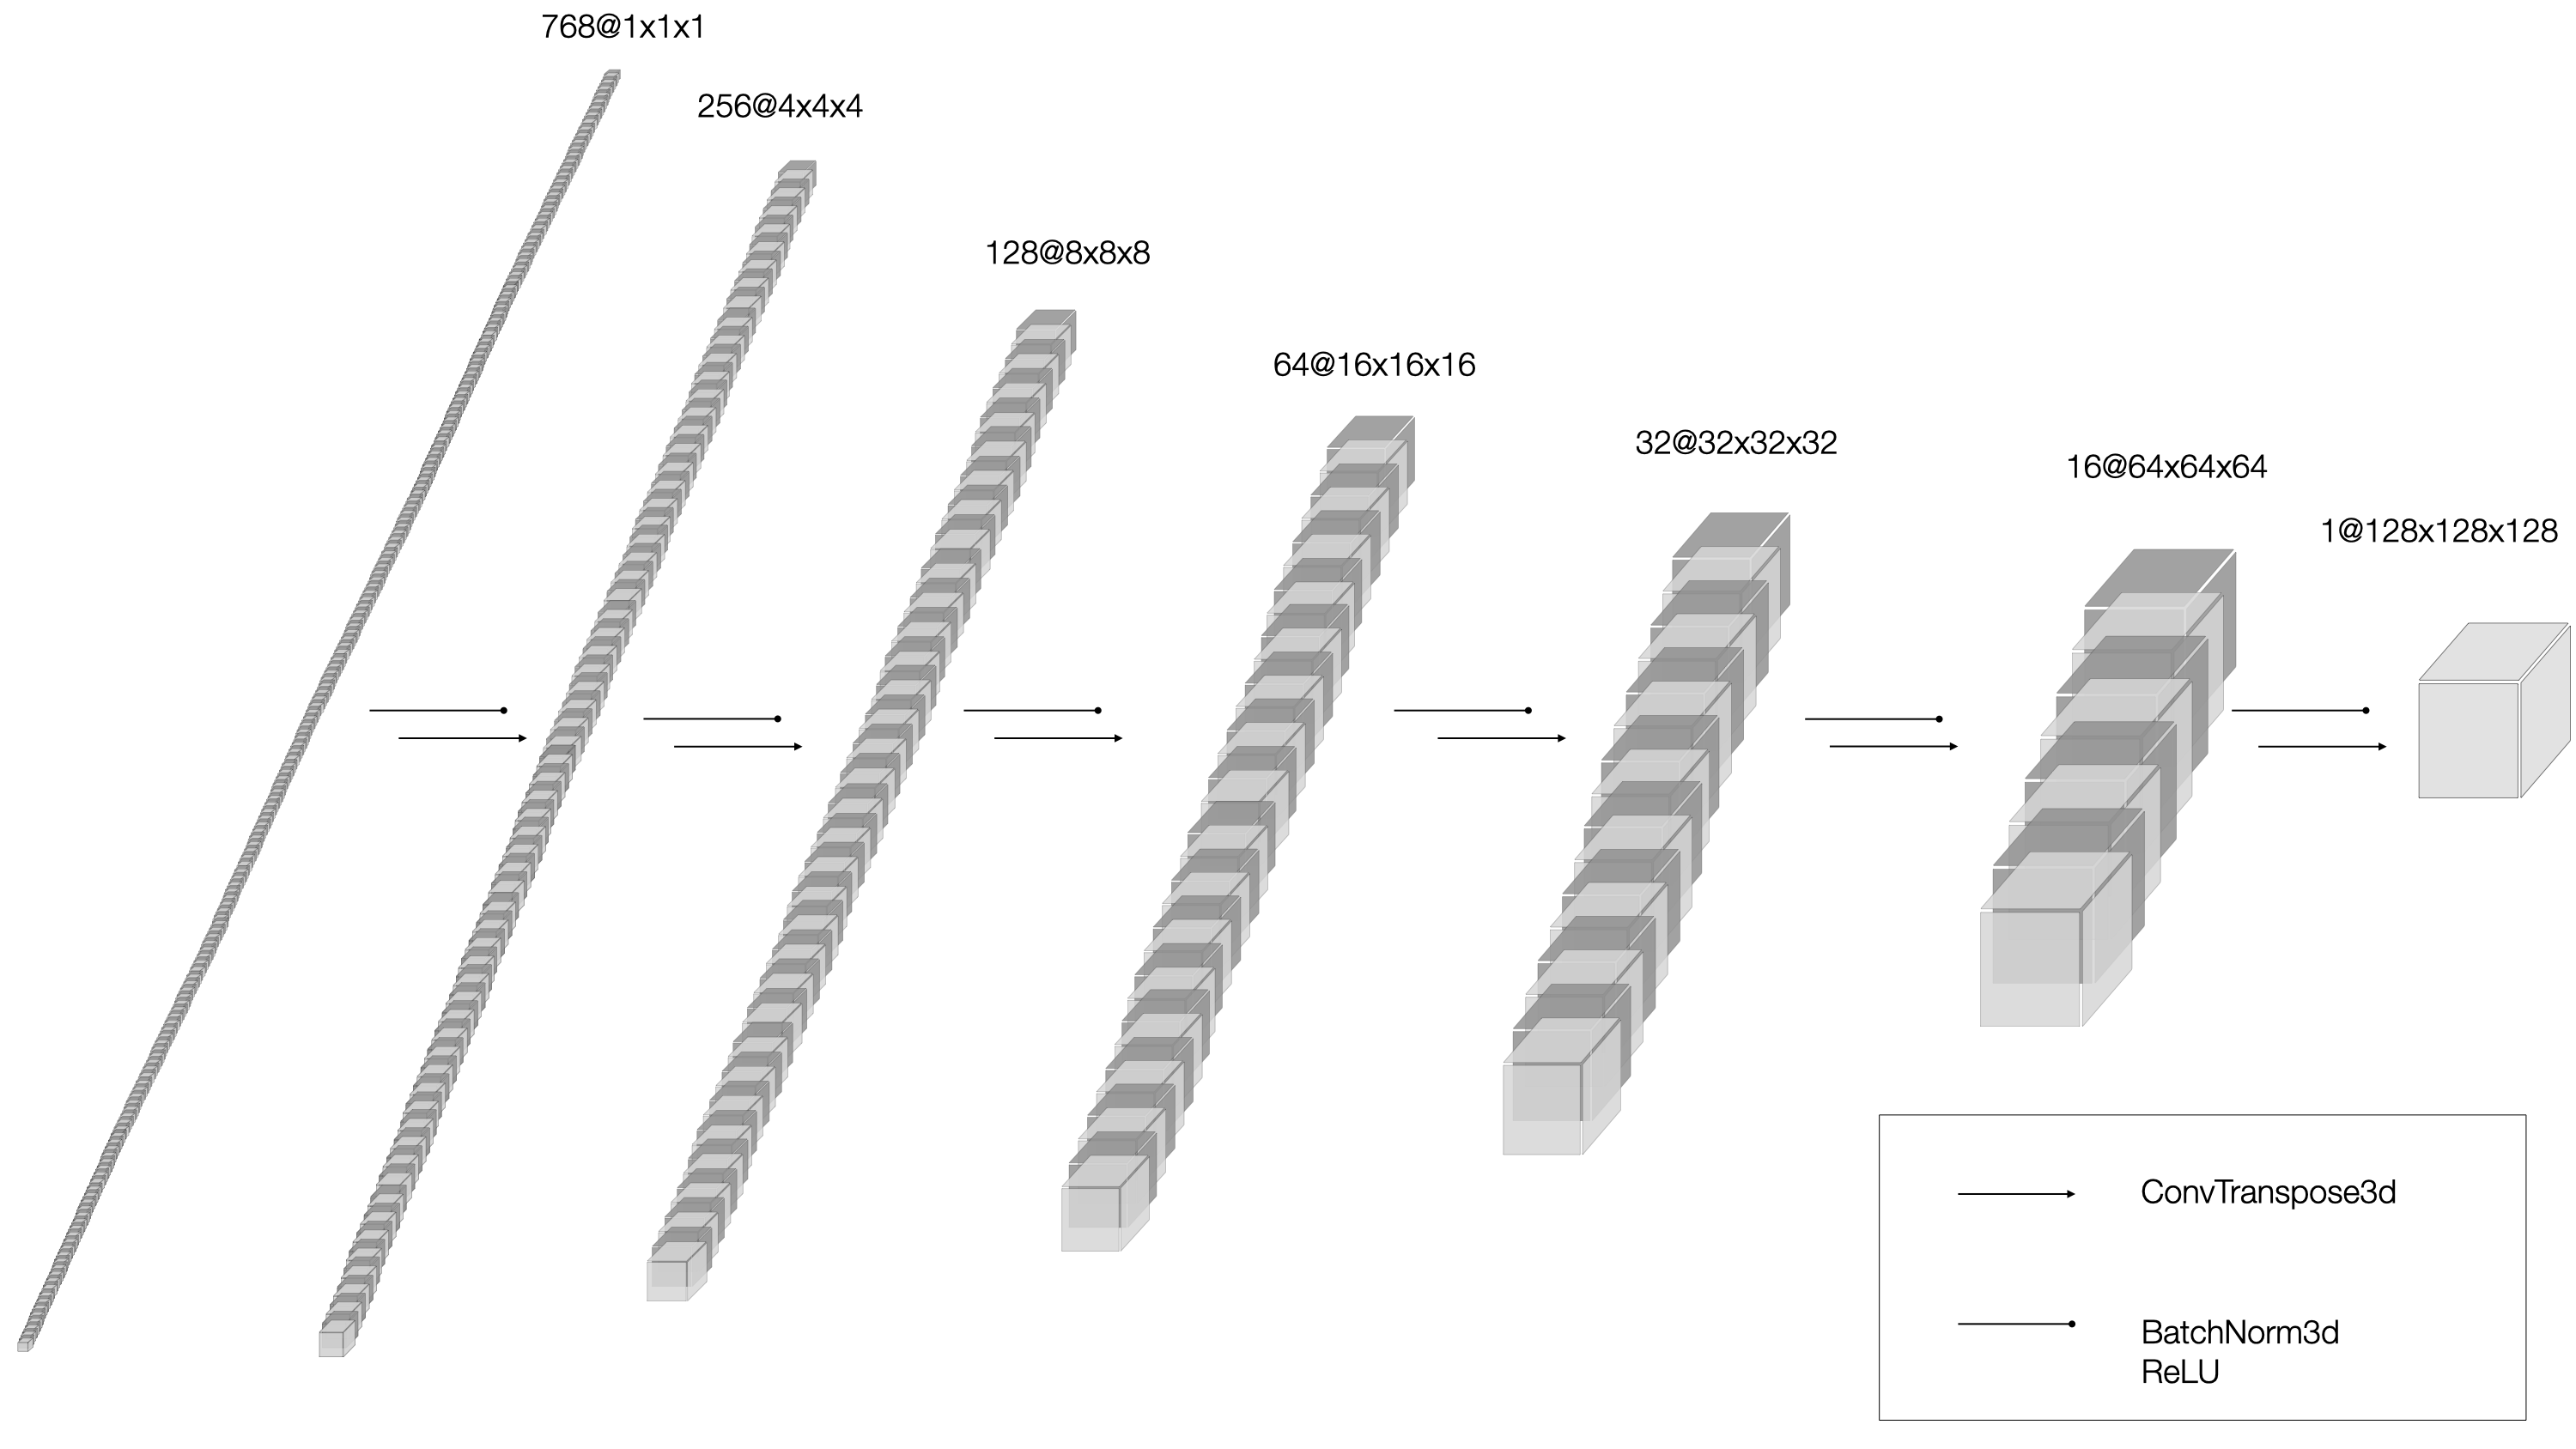
\includegraphics[width=0.8\textwidth]{figures/segmentation_decoder.001.png}
  \caption{Lightweight region-conditioned 3D mask decoder used for ASP.}
  \label{fig:seg_decoder}
\end{figure}

\clearpage
\subsection{Ablation Study on ASP Training}
\label{ablation_study}

We performed an ablation study to evaluate the main training choices used in ASP. For Alzheimer’s disease and epilepsy detection, we compared full fine-tuning (FF) with LoRA. As shown in Table~\ref{tab:sc_LoRA_classification}, both methods performed similarly for Alzheimer’s disease, while LoRA improved epilepsy detection. For age estimation, we additionally evaluated several ASP training ablations, including removing MAE alternation, encoder freezing, MAE-only pretraining, and training from scratch. The results in Table~\ref{tab:healthy_aging_results} correspond to the variants shown in Figure~\ref{fig:ASP}(e). We evaluate age estimation on UK Biobank as the internal test cohort and NACC as the external test cohort. To avoid confusion with masked autoencoding, we report mean absolute error as ``absolute error'' in the table.

The full ASP model achieves the best performance on both cohorts. Removing alternating masked-autoencoder reconstruction updates reduces performance, and removing both alternating updates and the initial encoder-freezing stage reduces it further. The masked-autoencoder-only model remains a strong baseline, but it is outperformed by the ASP variants that add anatomical supervision. Training from scratch performs worst, showing that ASP benefits from starting from a pretrained masked autoencoder.


\begin{table}[h]
\centering
\small
\begin{tabular}{cccc}
\toprule
\textbf{Task} & \shortstack[c]{\textbf{Evaluation}\\\textbf{Setting}} & \textbf{ASP (FF)} & \textbf{ASP (LoRA)} \\
\midrule

% \multirow{1}{*}{Parkinson's Detection}
% & Internal
% & 0.6549
% & \textbf{0.6997} \\
% \midrule

\multirow{8}{*}{\shortstack[c]{AD\\(Train: ADNI)}}
& ADNI   & 0.7800 & \textbf{0.7815} \\
& NACC   & 0.8260 & \textbf{0.8264} \\
& AIBL   & \textbf{0.8318} & 0.8232 \\
& OASIS1 & \textbf{0.8733} & 0.8083 \\
& OASIS2 & 0.8092 & \textbf{0.8439} \\
& OASIS3 & \textbf{0.7454} & 0.7376 \\
& OASIS4 & \textbf{0.6622} & 0.6457 \\
& MIRIAD & 0.9815 & \textbf{0.9866} \\
\midrule

\multirow{8}{*}{\shortstack[c]{AD\\(Train: NACC)}}
& ADNI   & \textbf{0.7676} & 0.7665 \\
& NACC   & 0.8438 & \textbf{0.8570} \\
& AIBL   & \textbf{0.8314} & 0.8216 \\
& OASIS1 & 0.9091 & \textbf{0.9120} \\
& OASIS2 & 0.8105 & \textbf{0.8308} \\
& OASIS3 & \textbf{0.7748} & 0.7658 \\
& OASIS4 & \textbf{0.6658} & 0.6502 \\
& MIRIAD & \textbf{0.9942} & 0.9914 \\
\midrule

\multirow{2}{*}{\shortstack[c]{Epilepsy Detection}}
& Internal & 0.6398 & \textbf{0.7507} \\
& External & 0.8359 & \textbf{0.8716} \\
\bottomrule
\end{tabular}
\caption{Comparison of ASP (FF/Full-Finetuning) and ASP (LoRA) AUROC performance across classification tasks.}
\label{tab:sc_LoRA_classification}
\end{table}

\begin{table*}[h!]
\centering
\scriptsize
\setlength{\tabcolsep}{4pt}
\renewcommand{\arraystretch}{1.15}
\resizebox{0.92\textwidth}{!}{%
\begin{tabular}{lccc ccc}
\toprule
\multirow{2}{*}{\textbf{Model}} 
& \multicolumn{3}{c}{\textbf{Internal: UK Biobank}} 
& \multicolumn{3}{c}{\textbf{External: NACC}} \\
\cmidrule(lr){2-4} \cmidrule(lr){5-7}
& \textbf{Pearson $r \uparrow$} 
& \textbf{MSE $\downarrow$} 
& \textbf{Abs. error $\downarrow$}
& \textbf{Pearson $r \uparrow$} 
& \textbf{MSE $\downarrow$} 
& \textbf{Abs. error $\downarrow$} \\
\midrule

\textbf{ASP (LoRA)}
& \textbf{0.9361} & \textbf{10.38} & \textbf{2.54}
& \textbf{0.8589} & \textbf{29.26} & \textbf{4.19} \\

ASP (Full-Finetuning)
& 0.9333 & 10.83 & 2.60
& 0.8464 & 32.06 & 4.32 \\

No masked-autoencoder alternation
& 0.9291 & 11.49 & 2.67
& 0.8324 & 34.51 & 4.46 \\

No alternation and no freezing
& 0.9220 & 12.59 & 2.78
& 0.7987 & 40.50 & 4.71 \\

Masked autoencoder only
& 0.9159 & 13.61 & 2.89
& 0.8043 & 45.35 & 5.20 \\

From scratch
& 0.8736 & 19.88 & 3.51
& 0.7407 & 55.84 & 5.79 \\

\bottomrule
\end{tabular}%
}
\caption{ASP training ablation evaluated on age estimation. Absolute error denotes mean absolute error in years.}
\label{tab:healthy_aging_results}
\end{table*}

\clearpage


%%=============================================%%
%% For submissions to Nature Portfolio Journals %%
%% please use the heading ``Extended Data''.   %%
%%=============================================%%

%%=============================================================%%
%% Sample for another appendix section			       %%
%%=============================================================%%

%% \section{Example of another appendix section}\label{secA2}%
%% Appendices may be used for helpful, supporting or essential material that would otherwise 
%% clutter, break up or be distracting to the text. Appendices can consist of sections, figures, 
%% tables and equations etc.


\rev{
\section{Comparison with related anatomy-informed pretraining methods}\label{sec:related_work}

\begin{table}[h]
\centering
\caption{Comparison of ASP with related methods that use anatomical information for brain MRI pretraining.}%\revnote{Authors: please verify the backbone entries}
\label{tab:related_work}
\footnotesize
\begin{tabular}{p{2.1cm}p{2.0cm}p{2.9cm}p{3.0cm}p{2.6cm}}
\hline
Method & Backbone & Anatomical signal & Pretraining objective & Representation used downstream \\ \hline
QuickNAT~\citep{roy2019quicknat} & 2D fully convolutional network & FreeSurfer segmentations of unlabeled scans & Supervised segmentation, then finetuning on manual labels & Full segmentation network \\
API-MAE~\citep{wang2023improving} & ViT (MAE) & Atlas-based anatomical prior & Masked autoencoding with anatomy-guided masking & Encoder for tumor segmentation \\
DAMT~\citep{kim2024domain} & 3D Swin transformer & Brain parcellation and morphological measures & Multi-task pretraining from scratch with several self-supervised objectives & Encoder with task-specific heads \\
AnatCL~\citep{barbano2025anatomical} & 3D CNN & Regional anatomical measurements & Contrastive learning weighted by anatomical similarity & Global embedding \\
ASP (ours) & 3D ViT-B/16 & FreeSurfer segmentations of 39 grouped regions & Continued pretraining of a converged MAE: frozen-encoder decoder training, then segmentation alternated with MAE & Global ViT embedding; skip-free, prompt-conditioned decoder discarded after pretraining \\ \hline
\end{tabular}
\end{table}
}
\end{appendices}

%%===========================================================================================%%
%% If you are submitting to one of the Nature Portfolio journals, using the eJP submission   %%
%% system, please include the references within the manuscript file itself. You may do this  %%
%% by copying the reference list from your .bbl file, paste it into the main manuscript .tex %%
%% file, and delete the associated \verb+\bibliography+ commands.                            %%
%%===========================================================================================%%



\end{document}
